\documentclass[11pt]{article}
\usepackage[T1]{fontenc}
\usepackage{lmodern,microtype,amsmath,amssymb,amsthm,mathtools,xurl,booktabs}
\usepackage[a4paper,margin=28mm]{geometry}
\usepackage{tikz}
\usetikzlibrary{arrows.meta,calc,positioning}
\usepackage[colorlinks=true,linkcolor=blue!55!black,citecolor=blue!55!black,urlcolor=blue!55!black]{hyperref}
\setlength{\emergencystretch}{2em}
\numberwithin{equation}{section}
\newtheorem{theorem}{Theorem}[section]
\newtheorem{proposition}[theorem]{Proposition}
\newtheorem{lemma}[theorem]{Lemma}
\newtheorem{corollary}[theorem]{Corollary}
\theoremstyle{definition}\newtheorem{definition}[theorem]{Definition}
\theoremstyle{remark}\newtheorem{remark}[theorem]{Remark}
\newcommand{\ii}{\mathrm i}
\newcommand{\CC}{\mathbb C}
\newcommand{\tr}{\operatorname{tr}}
\newcommand{\stat}{\operatorname{stat}}
\title{Preferred longitudes of Conway tree complements}
\author{}\date{}
\begin{document}\maketitle
\begin{abstract}
We identify the preferred-longitude eigenvalue of the geometric meridian germ of an ordered Conway tree. Each physical quarter-turn edge contributes a rational factor, and the original writhe and crossing powers determine the remaining meridian monomial. Boundary isotropy first makes the discrepancy independent of the auxiliary variables. A constant-field calculation and regular reconstruction at every nonzero main parameter then exclude additional rational factors; the argument includes the split trace-zero fibers. An explicit cusp-path calculation fixes the monomial and a Seifert-surface frame calculation fixes the determinant-one sign. Inserting meridian-filled zero-crossing circles extends the formula to arbitrary strict product junctions, including adjacent bare junctions and a folded half-label edge. The proof concerns marked representations and classical stationary actions. It uses no invariant asymptotic or recurrence hypothesis.
\end{abstract}

\section{The marked curve and the theorem}\label{pl:introduction}
A meridian eigenvalue does not determine a preferred longitude merely by fixing its value and tangent at the complete cusp. A nonconstant rational factor could have the same value and first derivative there. The proof below first excludes all such factors, then uses the cusp tangent to determine an integer exponent. This separation is essential at main parameters where an ideal cell chart degenerates although the group representation remains regular.

\subsection{The original diagram and its peripheral curves}
Take an ordered two-string Conway construction: products stack two tangles in their recorded order, physical quarter-turns rotate the whole four-point boundary, and the prescribed cylindrical closing pairs the final endpoints. Its main strands must form one knot, including any component already closed inside a subtangle. A crossing circle is an auxiliary component bounding the specified disk with two main punctures. Its retained half twist is $\epsilon_v\in\{-1,0,1\}$; filling the primitive slope $\mu_v+p_v\lambda_v$ gives signed crossing power
\begin{equation}\label{pl:power} n_v=\epsilon_v-2p_v.\end{equation}
All product orders, disk basepaths and endpoint flags remain part of the diagram. The auxiliary circles are pairwise unlinked.

Group consecutive products with no intervening physical turn into junctions. An \emph{all-circle tree} has a crossing circle at every junction; its finite underlying graph has at least one edge. A \emph{bare junction} has none. The strict class is defined by a nonempty angle domain: each original leaf has $0<a<1/2$, and each retained binary product with inputs $x,y$ and output $b$ has
\begin{equation}\label{pl:strict} \max(x,y)<b<x+y<1.\end{equation}
The forced final flat product is replaced by its exact complementary-label pairing. Any binary resolution of a bare junction keeps its original order; its hidden unturned wires are not physical edges. These support statements and the unique strict stationary state are proved in \cite[Sections 2--4]{Profiles}. Retain the original knot/parity test. In the strict two-leaf knot case at least one retained disk is pure ($\epsilon=0$); the two-odd pattern is a link and is excluded.

Let $\mathcal E$ denote the physical quarter-turn edges. Their covariant angle label $x_e$ is the one shared by the two ends in the symmetric product action; its ordinary output label is $1-x_e$. Set $X_e=e^{2\pi\ii x_e}$. The main positive meridian has eigenvalue $M$. The recorded source flag is its $M^{-1}$ eigenline; throughout this paper $L$ is the inverse longitude eigenvalue on that line, equivalently the longitude eigenvalue on the $M$ line. At circle $v$ the selected primitive disk-longitude eigenvalue is $-Q_v$. We use eigenvalue ratios for projective representations, so its longitude similarity is $Q_v^2$.

\subsection{The exact geometric inputs}
\begin{proposition}[Companion inputs, with their scope]\label{pl:imports}
The following marked statements are used.
\begin{enumerate}
\item The all-circle edge equation
\begin{equation}\label{pl:T1}
(X_e+Q_v)(X_e+Q_v^{-1})(X_e+Q_w)(X_e+Q_w^{-1})
 =(X_e-1)^2(1-X_eM^2)(1-X_e/M^2)
\end{equation}
reconstructs the original ordered augmented group near its complete point $M=Q_v=1$, $X_e=\ii$. The full puncture-pair conjugacies, primitive words and selected global flag are those of \cite[Theorems 1.1 and 3.1]{Nonparabolic}. In particular
\begin{equation}\label{pl:T3}
 e^{U_v}=Q_v^{-\epsilon_v}\prod_{e\ni v}\frac{Q_v+X_e}{1+Q_vX_e},\qquad V_v=2\log Q_v.
\end{equation}
The rational character formulas and their full ordered conjugacies, not only their traces, are part of this input.
\item The strict construction has its original positive complete geometry, actual white and shaded maps, primitive collar paths and sufficiently long independently signed fillings, as in \cite[Theorems 1.2--1.3 and Sections 6--8]{StrictGeometry}. Fixed crossing counts, including all their signs, are chosen before considering a deformation. The main cusp remains unfilled.
\item At a positive filled endpoint in the \emph{original augmented} triangulation, fixed primitive slope logarithms and the main meridian logarithm give the full local decorated representation germ. Thus the filled germ is smooth of dimension one, with coordinate $\log M$. This is the positive augmented germ statement of \cite[Theorem 1.2 and Proposition 6.1]{Nonparabolic}. A reconstructed representation must first be identified with that endpoint; slope eigenvalues alone do not supply the anchor. No positive triangulation of a newly drilled bare-junction diagram is required.
\end{enumerate}
\end{proposition}
These inputs identify the group representation and its metric; none asserts a main preferred-longitude formula. Section~\ref{plb:exact-elimination-of-the-angular-action} also uses the finite turn and multiplication identities of \cite[Proposition 3.2 and Theorem 3.3]{Newton}, the scalar factorial estimate of \cite[Lemma 5.2]{Newton}, and the exact Fourier trace of \cite[Lemma 6.1]{SourceBounds}. It does not use the later color-loss theorem in that paper or an asymptotic of a knot invariant.

\begin{theorem}[All-circle longitude]\label{pl:all-circle}
For the literal all-circle tree, put
\begin{equation}\label{pl:f}
 f_e=\frac{M^2-X_e}{1-M^2X_e},\qquad
 a_{\rm aug}=-w_\epsilon-\sum_v\epsilon_v.
\end{equation}
Here $w_\epsilon$ is the oriented writhe of the retained-crossing augmented diagram. On the integral source variety, the preferred main-longitude ratio satisfies
\begin{equation}\label{pl:T4} L_{\rm aug}^2=M^{2a_{\rm aug}}\prod_e f_e^2.\end{equation}
After the original disk fillings, its preferred filled peripheral word satisfies
\begin{equation}\label{pl:T6} L_{\rm fill}^2=M^{2a(D)}\prod_e f_e^2,
\qquad a(D)=-w(D)-\sum_v n_v.\end{equation}
This is a rational identity for that word before imposing fillings. On a connected geometric germ anchored at the actual complete hyperbolic filled knot it has the determinant-one form
\begin{equation}\label{pl:T7}
 \boxed{L_{\rm geom}(M)=-M^{a(D)}\prod_e\frac{M^2-X_e(M)}{1-M^2X_e(M)}.}
\end{equation}
The branch retains the original logarithms $U_v+p_vV_v=-2\pi\ii$. If one uses only the exponentiated equations, descent to the filled group additionally needs $Q_v^2\ne1$ at every filled circle, or the actual slope-word identity. A parabolic word with eigenvalue ratio one is not necessarily identity.
\end{theorem}

\begin{theorem}[Bare junctions and the original strict action]\label{pl:strict-longitude}
For every fixed strict ordered construction with the original knot qualification and sufficiently long independently signed original fillings, formula~\eqref{pl:T7} holds on its geometric meridian germ. The product is over its original physical edges, including edges between bare junctions. No restriction is imposed on bare-junction valence or adjacency.

More precisely, put $M=e^{\pi\ii t}$ and
$J(x)=\int_0^x\log(2\sin\pi r)\,dr$, continued from $0<x<1$. If $\Phi$ is the classical joint first-charge action of the same construction at $M=1$, the continued stationary branch is that of
\begin{equation}\label{pl:deformed-action}
 \Phi_t=\Phi+\sum_{e\in\mathcal E}
 [2J(x_e)-J(x_e+t)-J(x_e-t)]+\frac{\pi\ii a(D)}2t^2.
\end{equation}
Each circle contributes $\sum_{e\ni v}b(x_e,\tau_v)+\ii n_v\tau_v^2/(4\pi)-\ii\tau_v$, with $b$ defined in \eqref{plb:4}; each bare hub contributes the optimized sum of its original cubic gate actions~\eqref{plb:13}. Each physical edge has its one shared variable. This defines $\Phi$ with its constants and primitive first charge. Hidden binary-resolution variables may equivalently be retained before stationarity.
\end{theorem}
The proof identifies this classical critical branch with the original group representation; it makes no quantum estimate. In particular it does not assert an annihilator, an $A$-polynomial equality or a volume limit.

\section{Boundary isotropy and the edge differential}\label{pl:boundary-isotropy-and-the-edge-differential}

\subsection{The edge equation and a closed differential}\label{pl:the-edge-equation-and-a-closed-differential}

For an edge with endpoint variables \(Q,P\), let \(X\) satisfy

\begin{equation}\label{pl:R1}
(X+Q)(X+Q^{-1})(X+P)(X+P^{-1})
      =(X-1)^2(1-XM^2)(1-X/M^2).
\end{equation}

The variables are nonzero. We work first where all displayed factors
are nonzero and the selected root is simple. Write

\begin{equation}\label{pl:R2}
\begin{gathered}
 u=\log M,\quad q=\log Q,\quad p=\log P,\quad z=\log X,\\
 f=\frac{M^2-X}{1-M^2X},\quad
 \rho_Q=\frac{Q+X}{1+QX},\quad
 \rho_P=\frac{P+X}{1+PX}.
 \end{gathered}
\end{equation}

Only the differentials of the logarithms will be used. Their branches
therefore do not affect the identities below.

Let \(F\) be the logarithm of the quotient of the two sides of
\eqref{pl:R1}, holding \(z,q,p,u\) independent before differentiating.
Direct differentiation gives

\begin{equation}\label{pl:R3}
F_u=2(\log f)_z,\qquad
 F_q=-(\log\rho_Q)_z,\qquad
 F_p=-(\log\rho_P)_z.
\end{equation}

On the edge surface \(dF=0\). Moreover \(f\) has no direct
\(q,p\) dependence, and each \(\rho\) has no direct
\(u\) dependence or dependence on the other endpoint. Thus

\begin{equation}\label{pl:R4}
\begin{aligned}
 &du\wedge d\log f+
   \tfrac12d\log\rho_Q\wedge dq+
   \tfrac12d\log\rho_P\wedge dp\\
 &\quad=\tfrac12(F_u\,du+F_q\,dq+F_p\,dp)\wedge dz=0.
 \end{aligned}
\end{equation}

This proof uses the rational equation itself. It does not identify a
geometric volume by comparing numerical critical values. Since \eqref{pl:R4} is
an identity of rational differential forms, it holds on every smooth
part of the same algebraic component.

\subsection{The actual boundary pairing}\label{pl:the-actual-boundary-pairing}

The marked reconstruction input in Proposition~\ref{pl:imports} has assembled the ordered pieces into a representation
of the original augmented link exterior. Let \(L\) be the
eigenvalue of its preferred main longitude on the main
\(M\)-eigenline. At each auxiliary circle let \(U_v\) be the
logarithm of the primitive meridian similarity, and let the selected
longitude eigenvalue be \(-Q_v\). The exact local construction and
the original half-twist convention give

\begin{equation}\label{pl:R5}
U_v=\sum_{e\ni v}\log\rho_{v,e}-\epsilon_v\log Q_v,
 \qquad \epsilon_v\in\{-1,0,1\},
\end{equation}

up to locally constant logarithmic periods. The summands and the
primitive word must be established by the actual boundary gluing.

The infinitesimal boundary pairing is

\begin{equation}\label{pl:R6}
du\wedge d\log L+
             \tfrac12\sum_v dU_v\wedge d\log Q_v=0.
\end{equation}

Here all tori use the meridian--longitude orientations induced by the
same oriented exterior. The factor one half occurs because \(U_v\)
is a logarithm of an eigenvalue ratio, whereas \(\log Q_v\) is
a logarithm of a single determinant-one eigenvalue.

For completeness, \eqref{pl:R6} has a direct topological proof. Infinitesimal
variations of a representation are one-cocycles with values in its
adjoint local system. Pair two such cocycles by
\(\operatorname{tr}(XY)\) and take their cup product. The result
is a closed ordinary two-cochain, because the trace pairing is
invariant under conjugation. Its total evaluation on the boundary
of a fundamental three-chain is zero by the cochain Stokes identity.
On a torus with commuting diagonal holonomies, write their logarithms
as \(x\operatorname{diag}(1,-1)\) and
\(y\operatorname{diag}(1,-1)\). The alternating trace pairing
is \(2(dx\wedge dy)\). Summing over the boundary tori gives
\(\sum dx\wedge dy=0\). Substitute
\((x,y)=(u,\log L)\) at the main torus and
\((x,y)=(U_v/2,\log Q_v)\) at the auxiliary tori. This proves
\eqref{pl:R6} where the peripheral matrices are diagonalizable. The rational
identity extends over the remaining points where its terms are defined.

Subtract the sum of \eqref{pl:R4} over all edges from \eqref{pl:R6}. The half-twist term
in \eqref{pl:R5} has zero wedge product with \(d\log Q_v\). The result is

\begin{equation}\label{pl:R7}
du\wedge d\log\left(\frac{L}{\prod_e f_e}\right)=0.
\end{equation}

In particular, the discrepancy has no infinitesimal dependence on any
auxiliary variable. To avoid choosing determinant-one lifts globally,
use the squared discrepancy

\begin{equation}\label{pl:R8}
R=\frac{L^2}{\prod_e f_e^2}.
\end{equation}

It is a rational function whenever the original projective peripheral
representation is rational on the source variety: \(L^2\) is the
ratio of the two eigenvalues of the main longitude, with its ordered
main flag retained.

\section{The constant field of the source equations}\label{pl:the-constant-field-of-the-source-equations}

\subsection{Why the discrepancy is rational in the main meridian}\label{pl:why-the-discrepancy-is-rational-in-the-main-meridian}

Let \(k=\mathbb C(M)\), and let the graph have distinct unordered
edges. In particular this applies to a tree. The edge quadratic
gives, on putting \(Z=X+X^{-1}\):

\begin{equation}\label{pl:R9}
Z=\frac{2(M^2+M^{-2})-(Q+Q^{-1})(P+P^{-1})}
 {Q+Q^{-1}+P+P^{-1}+M^2+M^{-2}+2}.
\end{equation}

Work on the open set where these denominators are invertible; it
contains the complete branch. The squareclass of \(Z^2-4\) is

\begin{equation}\label{pl:R10}
H_e=(Q_v-1)^2(Q_w-1)^2
                  -4(M+M^{-1})^2Q_vQ_w.
\end{equation}

To see that the edge squareclasses are independent, extend the
coefficient field to an algebraic closure \(\overline{k}\).
Put \(t=(M+M^{-1})^2\ne0\) in this field. As a quadratic in
\(Y\), the polynomial
\((X-1)^2(Y-1)^2-4tXY\) has discriminant

\begin{equation}\label{pl:R11}
16tX[X^2+(t-2)X+1].
\end{equation}

Its order of vanishing at \(X=0\) is one, so it is not a square
in \(\overline{k}(X)\). Its coefficients in \(Y\) have no
common factor: at \(X=1\) the middle coefficient is \(-4t\).
It is therefore irreducible in \(\overline{k}[X,Y]\).

Different edges give different such prime polynomials, since they
involve different pairs of independent vertex variables. The valuation
at the prime \(H_e\) is odd for its own squareclass and zero for
every other edge. Hence every nonempty product of edge squareclasses
is nonsquare. Adjoining their square roots has degree \(2^{|\mathcal E|}\)
even after extending \(k\) to \(\overline{k}\). This proves
geometric integrality of the generic source fiber over \(M\).
In particular \(k\) is algebraically closed in its function
field \(\mathcal F\).

The logarithmic derivatives in all the \(Q_v\) extend uniquely
to the finite separable field \(\mathcal F\). If an element of
\(\mathcal F\) is killed by every such derivative, its relative
differential over \(k\) vanishes. In characteristic zero it is
algebraic over \(k\), and therefore belongs to \(k\) by the
preceding paragraph. Applying this to \eqref{pl:R7}--\eqref{pl:R8} gives

\begin{equation}\label{pl:R12}
R\in\mathbb C(M)^*.
\end{equation}

The specialization of \eqref{pl:R10} at \(M=\pm i\) is a square. This
does not invalidate the generic integrality proof; it does mean that
those fibers need the separate check in Section~\ref{pl:regular-reconstruction-at-every-nonzero-main-value}.

\section{Regular reconstruction at every nonzero main value}\label{pl:regular-reconstruction-at-every-nonzero-main-value}

\subsection{A uniform algebraic open set in every fiber}\label{pl:a-uniform-algebraic-open-set-in-every-fiber}

For one edge write

\begin{equation}\label{pl:G1}
m=M^2,\quad D=m+m^{-1},\quad
 \beta=Q+Q^{-1},\quad\gamma=P+P^{-1},\quad
 S=\beta+\gamma+D+2.
\end{equation}

Use \(X\) for the source wire coordinate. Its equation is the
quadratic

\begin{equation}\label{pl:G2}
F(X)=S(X^2+1)+(\beta\gamma-2D)X=0.
\end{equation}

This is equivalent, on \(X\ne0\), to the original degree-four
effective edge equation after its cancellation. Define

\begin{equation}\label{pl:G3}
J=\beta\gamma-2\beta-2\gamma-4D-4.
\end{equation}

The discriminant of \eqref{pl:G2} is

\begin{equation}\label{pl:G4}
\Delta=(\beta+2)(\gamma+2)J.
\end{equation}

Consider the open conditions

\begin{equation}\label{pl:G5}
\begin{gathered}
 QP\ne0,\qquad
 (\beta+2)(\gamma+2)(\beta+D)(\gamma+D)\ne0,\\
 S\ne0,\qquad \Delta\ne0.
\end{gathered}
\end{equation}

For every fixed \(M_0\in\mathbb C^*\), these conditions define
a nonempty Zariski open subset of the \(Q,P\) torus. Indeed each
excluded expression is a nonzero polynomial in the independent
variables \(\beta,\gamma\). For a fixed finite tree the same
conditions can be imposed simultaneously at every edge, since
their product is again a nonzero Laurent polynomial in the
vertex parameters \(Q_v\).

On \eqref{pl:G5}, both roots of \eqref{pl:G2} are finite, nonzero and distinct.
Several useful evaluations are

\begin{equation}\label{pl:G6}
\begin{aligned}
 F(1)&=(\beta+2)(\gamma+2),&
 F(-1)&=-J,\\
 F(m)&=m(\beta+D)(\gamma+D),&
 F(m^{-1})&=m^{-1}(\beta+D)(\gamma+D).
\end{aligned}
\end{equation}

Hence neither root is \(1,-1,m,m^{-1}\). In particular

\begin{equation}\label{pl:G7}
f=\frac{m-X}{1-mX}
\end{equation}

is a finite nonzero function at every point under consideration.
The auxiliary factors \((Q+X)/(1+QX)\) and
\((P+X)/(1+PX)\) are also finite and nonzero. To see this,
substitute \(X=-Q\) or \(X=-Q^{-1}\) in the original edge
equation. A zero can occur only when \(Q=-1\) or
\(Q=-m^{\pm1}\), excluded by \eqref{pl:G5}; the other endpoint is
identical.

\subsection{The actual character matrices remain regular}\label{pl:the-actual-character-matrices-remain-regular}

Put \(t=M+M^{-1}\), \(p=-\beta\), \(q=-\gamma\), and
\(\mathcal X=2+SX\). The character adapter uses

\begin{equation}\label{pl:G8}
A=\begin{pmatrix}M&1\\0&M^{-1}\end{pmatrix},\qquad
 B=\begin{pmatrix}M^{-1}&0\\p-2&M\end{pmatrix}.
\end{equation}

Its matrix \(C\) is given by

\begin{equation}\label{pl:G9}
\begin{gathered}
 h=M-M^{-1},\qquad
 c=\frac{M\mathcal X+M^{-1}q-2t}{D-p},\\
 d=\frac{q-M^2-1+hc}{p-2},\qquad
 e=\mathcal X-1-M^{-2}-hc,\qquad
 C=\begin{pmatrix}c&d\\e&t-c\end{pmatrix},\\
                         D_0=(ABC)^{-1}.
\end{gathered}
\end{equation}

The only denominators in \eqref{pl:G8}--\eqref{pl:G9}, besides powers of \(M\),
are \(p-2=-(\beta+2)\) and \(D-p=D+\beta\).
They are units on \eqref{pl:G5}. The four matrices have determinant one
and trace \(t\), with
\(\operatorname{tr}(AB)=-\beta\) and
\(\operatorname{tr}(BC)=-\gamma\), by \eqref{pl:G2}.
The formulas contain no division by \(M-M^{-1}\) or by \(t\).

The pure auxiliary transports are

\begin{equation}\label{pl:G10}
V=AB-\frac{1+X(\beta+1)}{1-X}I,\qquad
 T=BC+\frac{X+\gamma+1}{1-X}I.
\end{equation}

They satisfy the full puncture conjugacies, not just the trace
equations. Their determinants simplify on \eqref{pl:G2} to

\begin{equation}\label{pl:G11}
\det V=\frac{X(\beta+2)^2(\beta+D)}{S(X-1)^2},\qquad
 \det T=\frac{X(\gamma+2)^2(\gamma+D)}{S(X-1)^2}.
\end{equation}

For example the first determinant before reduction is
\[
 \frac{(\beta+2)(X^2+\beta X+1)}{(X-1)^2}.
\]
Equation \eqref{pl:G2} implies
\(X+X^{-1}+\beta=(\beta+2)(\beta+D)/S\), giving \eqref{pl:G11}.
The second computation is the same with \(\gamma\).
Thus both full transport matrices and their inverses are regular
on \eqref{pl:G5}, on either root of the source equation.

Every disk boundary pair is irreducible there. For the first
pair the standard direct trace calculation gives

\begin{equation}\label{pl:G12}
\operatorname{tr}[A,B]-2=(\beta+2)(\beta+D)\ne0.
\end{equation}

The second has the corresponding \(\gamma\) formula.
One can also derive \eqref{pl:G12} directly from the two matrices \eqref{pl:G8}.
For determinant-one two-generator representations this
nonzero expression excludes a common invariant line. In
particular neither generator is central.

The positive odd collar uses \(H=P_{\mathrm{disk}}^{-1}-I\)
with the original ordered disk product. Since
\(\operatorname{tr}P_{\mathrm{disk}}=-\beta\),

\begin{equation}\label{pl:G13}
\det H=2+\beta\ne0.
\end{equation}

The same holds at the other endpoint. The actual positive and
negative Hurwitz generators and all fixed powers remain
invertible. Thus odd seams introduce no exceptional fixed
value of \(M\).

\subsection{Sewing finitely many blocks uses a rational finite atlas}\label{pl:sewing-finitely-many-blocks-uses-a-rational-finite-atlas}

The ordered page construction glues two boundary pairs whose
matrices are explicit rational functions of the edge variables.
Their identification is the actual one in the native table;
where a loop is inverted or its order reversed, that operation
is included before asking for an intertwiner.

After those marked identifications, the two ordered boundary
pairs have the same three traces and are irreducible by \eqref{pl:G12}.
Their intertwiner is the solution line of

\begin{equation}\label{pl:G14}
G a=a'G,\qquad G b=b'G.
\end{equation}

The solution line is one-dimensional, and every nonzero solution
is invertible. Indeed a nontrivial kernel or image would be an
invariant line for one of the two irreducible pairs. Existence
can be proved without using ideal vertices. For an irreducible
pair the four matrices \(I,a,b,ab\) span
\(\operatorname{Mat}_2\). Their multiplication table is
determined by the common trace \(t\) and product trace \(p\):

\begin{equation}\label{pl:G14a}
a^2=ta-I,\quad b^2=tb-I,\quad
 ab+ba=t(a+b)+(p-t^2)I.
\end{equation}

The same table for the primed pair gives an isomorphism of
the two full matrix algebras, hence conjugation by an
invertible matrix. Equivalently put both pairs in the
explicit form \eqref{pl:G8}; irreducibility ensures that the two
selected generator flags are distinct and that the
off-diagonal entry used to normalize the frame is nonzero.
Either proof retains the ordered generators, not just the
individual conjugacy classes.

Equation \eqref{pl:G14} is a finite linear system with rational entries.
Choose a nonzero maximal minor and normalize one coordinate
on its one-dimensional kernel. This gives a rational
intertwiner regular in a neighborhood of that point.
No single choice of minor has to work at all parameters.
The finitely many choices form a rational atlas; the resulting
representation and peripheral eigenvalue ratios are independent
of the scalar normalization of an intertwiner.

Start with one edge block. The actual page insertion joins each
new block to the preceding union along one marked disk side.
Its attaching graph is a tree of blocks, so this inductively
constructs a representation of the entire page-cut object with
all matrices regular. The distinguished pure or odd seam at
each circle is then installed using \eqref{pl:G10}, \eqref{pl:G13}, and the two
full generator conjugacies of its actual mapping cylinder.
Those formulas preserve its outer disk product. Van Kampen
therefore gives the representation of the original augmented
exterior. No arbitrary pants permutation or commutativity of
tangles is used.

For any fixed finite tree, intersecting the finitely many
necessary open charts gives a nonempty open set over the
fixed \(M_0\). Equivalently, at any good point one may choose
each nonzero intertwiner minor in succession, obtaining a
regular neighborhood of that point. This proves existence of
the required actual rational \(\mathrm{PGL}_2\) reconstruction
at every nonzero main parameter.

This step requires the actual marked boundary conjugacies,
not just a formal family of characters. They were identified
with the original cut in the page/collar proof and remain
rational identities on the present open sets.

\subsection{The exceptional-looking main parameters}\label{pl:the-exceptional-looking-main-parameters}

At \(M=\pm1\), one has \(D=2\). Conditions \eqref{pl:G5} simply
exclude \(\beta=-2,\gamma=-2\), together with the stated
nonzero discriminant and denominator. The main matrix in
\eqref{pl:G8} is a noncentral parabolic. Nothing in \eqref{pl:G8}--\eqref{pl:G14} divides
by its eigenvalue difference, so the reconstruction is regular.

At \(M=\pm i\), one has \(D=-2\). The source discriminant
becomes

\begin{equation}\label{pl:G15}
\Delta=(\beta^2-4)(\gamma^2-4).
\end{equation}

With \(\beta=Q+Q^{-1}\) and \(\gamma=P+P^{-1}\),
this is a square in \(\mathbb C(Q,P)\). The fiber therefore
splits; generic-fiber irreducibility must not be asserted
at these two values. Nevertheless \eqref{pl:G5} gives two distinct
simple roots at generic \(Q,P\), and all matrices \eqref{pl:G8}--\eqref{pl:G14}
are regular. The main punctures are semisimple, with
eigenvalues \(i,-i\) or \(-i,i\), and remain noncentral.
The two roots can be written explicitly as

\begin{equation}\label{pl:G15a}
X=-\frac{Q+P}{1+QP},\qquad
             X=-\frac{1+QP}{Q+P}.
\end{equation}

For generic \(Q,P\) they differ and avoid \(1,-1\).
Fixing these auxiliary values, the implicit-function theorem
for \eqref{pl:G2} therefore continues either root holomorphically in
\(M\) through \(M_0=i\) or \(-i\).

The native ideal cell chart explains a possible false alarm.
At \(m=-1\), its preliminary white coordinate \(E_0\)
satisfies

\begin{equation}\label{pl:G16}
(E_0P-E_0Q-PQ+1)(E_0PQ-E_0-P+Q)=0.
\end{equation}

On one branch the two minus-copy circle apices coincide; on
the other the plus-copy apices coincide. Thus that particular
eight-tetrahedron ideal subdivision degenerates. This does
not make the actual group matrices singular: \eqref{pl:G8}--\eqref{pl:G14} are
an explicit regular reconstruction at precisely those points.
The rigidity argument needs the latter, not a positive
triangulation at every complex value of \(M\).

\subsection{A regular nonzero main eigenvalue ratio}\label{pl:a-regular-nonzero-main-eigenvalue-ratio}

Every main peripheral word is a fixed finite product of the
regular invertible group matrices just constructed. Hence its
matrix and inverse are regular at the chosen point.
The main meridian is noncentral.

There is one important trace-zero detail. Commutation in
\(\mathrm{PGL}_2\) alone would allow a longitude to
exchange the two eigenlines of a trace-zero meridian.
Use the matrices on the local section through nearby \(M\).
Normalize the meridian \(\mu\) to determinant one.
Its projective commutation with a regular invertible
longitude representative \(L\) gives
\(L\mu L^{-1}=\kappa\mu\), where
\(\kappa^2=1\) by determinants. At the nearby parameters
with \(M+M^{-1}\ne0\), taking traces gives \(\kappa=1\).
Consequently the exact matrix identity

\begin{equation}\label{pl:G16a}
L\mu=\mu L.
\end{equation}

extends to the trace-zero point. The undesired
anticommuting component is not part of this continued
representation. This also follows as a rational identity
on the integral generic source family.

At \(M_0\ne\pm1\), choose
its specified eigenline locally; its eigenvalue on a commuting
peripheral word is finite and nonzero. The ratio of the two
peripheral eigenvalues is therefore a regular unit.

The same conclusion holds at \(M_0=\pm1\), without
diagonalizing the meridian. In a frame in which its
upper-right entry is a unit, a commuting matrix \(L\) has
the form

\begin{equation}\label{pl:G17}
L=aI+b\mu.
\end{equation}

Here \(b=L_{12}/\mu_{12}\) and
\(a=L_{11}-b\mu_{11}\) are regular. Its two selected
eigenvalues are \(a+bM\) and \(a+bM^{-1}\). Both are
nonzero at the point because \(\det L\ne0\).
Their ratio is therefore regular and nonzero through the
parabolic value. Scalar changes of the representative \(L\)
cancel from the ratio.

The selected meridian eigenline itself is regular as well:
in this frame it is spanned by
\((\mu_{12},M-\mu_{11})\), or by
\((\mu_{12},M^{-1}-\mu_{11})\) for the other selection.
The first coordinate is a unit, including at \(M=\pm1\).
Thus coalescence of the two flags does not create a pole in
the marked eigenvalue ratio.

This directly applies to the square of a determinant-one
preferred-longitude eigenvalue, with the chosen inverse
convention if necessary. It does not require choosing a
global square root of a projective matrix determinant.
Every factor \eqref{pl:G7}, and every framing monomial in \(M\),
is likewise a unit at the point.

\subsection{Local sections and the integral total family}\label{pl:local-sections-and-the-integral-total-family}

More concretely, fix generic numerical auxiliary values
\(Q_v=q_v\) satisfying all the open conditions at \(M_0\),
and choose a simple root of every edge equation. The implicit
function theorem gives simultaneous holomorphic roots
\(X_e(M)\) near \(M_0\). At the chosen point select a
nonzero minor in each linear gluing system \eqref{pl:G14}. Those same
minors remain nonzero nearby. All actual group matrices,
their inverses and the main eigenvalue ratio are then
holomorphic along this local section. This is stronger than
the existence of an isolated good point in a special fiber.

The split trace-zero fibers do not invalidate this argument.
Let \(B\) be the Laurent coordinate ring in \(M,Q_v\),
localized at all \(S_e\). Dividing \eqref{pl:G2} by \(S_e\) makes
every edge polynomial monic with constant term one. The
simultaneous source algebra is therefore free over \(B\),
with basis the products \(\prod_e X_e^{\epsilon_e}\),
\(\epsilon_e\in\{0,1\}\). The independent generic edge
squareclasses imply that its generic localization is a
single field of degree \(2^{|\mathcal E|}\). Freeness embeds the
source algebra into that field; in particular the total
source variety is integral and has no additional vertical
component. Its simple points at \(M=\pm i\) belong to
the closure of the same generic family. A rational identity
proved there therefore holds on the regular local section
just constructed.

\section{The actual preferred-cusp
translation}\label{pl:cusp}

We use the actual parabolic-main face maps in \cite[Section 7]{StrictGeometry}.
They also compute the cusp tangent of the all-circle family: at $M=1$
the native chart of \cite{Nonparabolic} has its preliminary white
coordinate equal to $X$, and its four white matrices are the matrices
below up to the stated projective normalizations. The full ordered disk
conjugacies identify the shaded transports as well. Alternatively, the
positive marked gluing germ identifies both constructions with the same
original complete holonomy for prescribed auxiliary longitude logs.
Both descriptions retain the same physical wire labels. Thus the
following calculation is of the actual main peripheral word, not a
comparison of critical values.

\subsection{Meridians, endpoint signs, and additive
displacement}\label{meridians-endpoint-signs-and-additive-displacement}

Normalize each ordered quadrilateral to
\((C_0,C_1,C_2,C_3)=(0,\infty,1,R)\), and put \(E=e^{2\pi i b}\). In
these charts, a white face is a piece of an original projection region;
the other, shaded faces are pieces of the crossing disks. Use the actual
white matrices \begin{equation}
\begin{aligned}
W_0&=\begin{pmatrix}1&0\\0&E\end{pmatrix},
&W_1&=\begin{pmatrix}1&E-1\\0&E\end{pmatrix},\\
W_2&=\begin{pmatrix}E-R&R(1-E)\\E-1&1-ER\end{pmatrix},
&W_3&=\begin{pmatrix}R&0\\1-E&ER\end{pmatrix}.
\end{aligned}
\label{plc:4}
\end{equation} At an open shaded boundary some of these are completion maps. The
marked geometry input in Proposition~\ref{pl:imports} proves that every occurrence used in the final
closed peripheral paths is supplied by the actual adjacent white face.

Set \(d_j=(-1)^j\) and \begin{equation}
\mu_j=(W_{j-1}^{-1}W_j)^{d_j}.
\label{plc:5}
\end{equation} The coordinates \begin{equation}
\begin{aligned}
\xi_0(z)&=\frac{ER}{(E-1)z},
&\xi_1(z)&=-\frac{z}{E-1},\\
\xi_2(z)&=-\frac{E(R-1)}{(E-1)(z-1)},
&\xi_3(z)&=-\frac{R(R-1)}{(E-1)(z-R)}
\end{aligned}
\label{plc:6}
\end{equation} send the corresponding corner to infinity and send \(\mu_j\) to
\(u\mapsto u+1\). These identities follow by multiplying \eqref{plc:4}.

The endpoint sign has a geometric meaning. Orient a main arc into its
leaf at corner \(j\). Its positively oriented small meridian is
\(\mu_j^{d_j}\); orient the arc out of the leaf and it is
\(\mu_j^{-d_j}\). This is the right-hand meridian convention in the
ordered projection chart \(0,1,2,3\): crossing one white sector and
returning through the preceding one gives \(W_{j-1}^{-1}W_j\) for an
inward arc. Formula \eqref{plc:5} therefore supplies exactly the displayed signs.
At infinity use the finite local coordinate \(1/z\). Reversing the
strand orientation reverses both its meridian and the direction of its
longitude.

Consider an open main arc from corner \(j\) to corner \(k\), including
its specified peripheral push-off. In the local coordinates its actual
transport has the form \begin{equation}
u_k=-d_jd_k\,u_j+\beta.
\label{plc:7}
\end{equation} The multiplier follows by transporting the same oriented meridian: it
is \(d_j\) times the local unit at the incoming endpoint and \(-d_k\)
times the local unit at the outgoing endpoint. Define the displacement
of this arc to be \begin{equation}
D_{\mathrm{arc}}=-d_k\beta.
\label{plc:8}
\end{equation} This definition does not depend on the direction in which the arc is
followed. The inverse affine map has translation \(-\beta/(-d_jd_k)\),
and its displacement is \(-d_j[-\beta/(-d_jd_k)]=-d_k\beta\). This
simultaneously reverses the path and the oriented meridian; it does not
add raw translations from incompatible meridian frames.

When two endpoints are joined by an actual identity segment, its
coordinate change from \(j\) to \(k\) has the same affine multiplier
\(-d_jd_k\). Its contribution is instead \begin{equation}
D_{\mathrm{join}}=d_k\beta.
\label{plc:9}
\end{equation} Here the path leaves the first arc and enters the next. The same
inverse-map calculation proves direction independence.

These displacements add under concatenation. For an arc \(i\to j\), a
joining segment \(j\to k\), and an arc \(k\to l\), write their shifts as
\(\beta_X,\beta_J,\beta_Y\). Multiplying the three affine maps gives
shift \begin{equation}
(-d_kd_l)(-d_jd_k)\beta_X
       +(-d_kd_l)\beta_J+\beta_Y.
\end{equation} Multiplying by \(-d_l\) gives exactly \begin{equation}
-d_j\beta_X+d_k\beta_J-d_l\beta_Y.
\label{plc:10}
\end{equation} The product multiplier is \(-d_id_l\), as required. The same identity
applies when a join creates a closed component. A closed component has
multiplier one and its displacement is its actual longitude translation
in the consistently oriented unit-meridian frame.

Let \(S(Q)\) be the sum of these displacements for the two open arcs and
any already closed main components inside a tangle. If a boundary
coordinate at a corner changes by \(u'_j=\alpha_j u_j+\beta_j\), with
\(\alpha_j=d_j/d'_j\), then \begin{equation}
S(Q')-S(Q)=-\sum_{\text{four endpoints }j}d'_j\beta_j.
\label{plc:11}
\end{equation} This follows from \eqref{plc:8}, once at each endpoint. Closed components do
not change. Equations \eqref{plc:7}--\eqref{plc:11} are a local chain lemma: they apply
regardless of how many odd leaves a component visits or which direction
is used to evaluate it.

For an open expression, this is boundary-chart bookkeeping in the
original two-ball cut, with its completion maps still labeled as such.
It does not declare its metric quadrilateral to be a physical
four-punctured tangle boundary or assign virtual white maps to new group
generators. The product identities transport this bookkeeping. At the
final closure every used white completion is the actual adjacent
original white transition, by the marked geometry input. Only then do the
assembled paths give the asserted closed peripheral words.

Equivalently, for any one step write
\(\xi_bF\xi_a^{-1}(w)=\kappa w+\beta\), and let the globally oriented
meridian be the local unit raised to \(\alpha_a,\alpha_b\in\{1,-1\}\).
Consistency is \(\alpha_b\kappa=\alpha_a\); the actual translation
contribution is \(\alpha_b\beta\). Reversing the traversal replaces the
shift by \(-\beta/\kappa\), and reversing the oriented meridian replaces
the target sign by \(-\alpha_a\). Their product is again
\(\alpha_b\beta\). Equations \eqref{plc:8} and \eqref{plc:9} are this rule at an arc and a
joining segment respectively. This explicitly includes the
multiplier-minus-one odd routes below.

\subsection{The exact product
potential}\label{the-exact-product-potential}

Define the boundary potential \begin{equation}
P(E,R)=\frac{E+R}{E-1},\qquad I(Q)=S(Q)-P(E,R).
\label{plc:12}
\end{equation} For the original ordered product prism we claim \begin{equation}
I(FG)=I(F)+I(G).
\label{plc:13}
\end{equation} This is an identity of actual coordinate transports, not an equality
of their absolute values.

Here is a rational verification retaining every translation. Write the
prism angle phases as \(a,b,c\), so its vertices are \begin{equation}
v_0=1,\quad v_1=a,\quad v_2=ab,\quad v_3=abc,\qquad
 P_*=
 1+a-a\,\frac{ab(1+c)-1-a}{a^2b^2c-a}.
\label{plc:14}
\end{equation} The lower, upper and output ordered quadrilaterals are
\((1,a,P_*,\infty)\), \((\infty,P_*,ab,abc)\), and \((1,a,ab,abc)\).
Their \(E\) parameters are \(bc,ab,abc\). Their normalized fourth
vertices are \begin{equation}
\begin{aligned}
 R_F&=\frac{a(b-1)(bc-1)}{(ab-1)(abc-1)},\\
 R_G&=\frac{c(b-1)(ab-1)}{(bc-1)(abc-1)},\\
 R_o&=\frac{(b-1)(abc-1)}{(ab-1)(bc-1)}.
\end{aligned}
\label{plc:15}
\end{equation} Apply \eqref{plc:6} after the unique normalized three-point map for each
quadrilateral. The two joining and four external rebasing maps all have
multiplier one. Their translations are \begin{equation}
\begin{array}{c|c}
F_2\longrightarrow G_1&bc/(bc-1)\\
F_3\longrightarrow G_0&-a(b-1)/[(ab-1)(abc-1)]\\
F_0\longrightarrow o_0&0\\
F_1\longrightarrow o_1&0\\
G_2\longrightarrow o_2&ab(c-1)/[(ab-1)(abc-1)]\\
G_3\longrightarrow o_3&(b-1)(c-1)/[(ab-1)(bc-1)(abc-1)].
\end{array}
\label{plc:16}
\end{equation} For example a world quadrilateral \((q_0,q_1,q_2,q_3)\) is normalized
by \((z-q_0)(q_2-q_1)/[(z-q_1)(q_2-q_0)]\), with the corresponding
limits at infinity. Inserting this map into \eqref{plc:6} gives \eqref{plc:16}.

By \eqref{plc:9} and \eqref{plc:11}, the correction \(S(FG)-S(F)-S(G)\) is minus the first
entry of \eqref{plc:16}, plus the second, minus the fifth and plus the sixth.
Substituting \eqref{plc:15} into \eqref{plc:12} gives exactly that expression: \begin{equation}
S(FG)-S(F)-S(G)
                  =P(abc,R_o)-P(bc,R_F)-P(ab,R_G).
\label{plc:17}
\end{equation} This proves \eqref{plc:13}. All variables in \eqref{plc:14}--\eqref{plc:17} are independent
wherever the displayed charts are nondegenerate. Thus the identity
continues to the original complex deformed branch. In particular hidden
binary resolutions inside a product hub contribute no uncancelled term.

\subsection{Turns and the final
closure}\label{turns-and-the-final-closure}

The actual quarter-turn is \begin{equation}
T_Q(z)=\frac{R-1}{z-1},\qquad
 (E,R)\longmapsto(E^{-1},1-R),\qquad j\longmapsto j-1.
\label{plc:18}
\end{equation} In the coordinates \eqref{plc:6}, the four rebasing maps have multiplier minus
one. In old corner order \(j=0,1,2,3\), their shifts are \begin{equation}
\frac{ER}{E-1},\quad-\frac1{E-1},\quad0,\quad\frac R{E-1}.
\label{plc:19}
\end{equation} Equation \eqref{plc:11} gives \(S(TQ)-S(Q)=(ER-R+1)/(E-1)\). Subtract the two
potentials in \eqref{plc:12}. The result is \begin{equation}
I(TQ)-I(Q)=\frac{2(E+1)}{E-1}=-2i\cot(\pi b).
\label{plc:20}
\end{equation} This calculation retains the minus multipliers in \eqref{plc:19}; summing their
shifts without \eqref{plc:11} would give the wrong sign.

At the final reverse-order closing gluing, the two input parameters are
\((E,R)\) and \((E^{-1},R)\), and the actual map from the second to the
first is \begin{equation}
C_Q(z)=\frac{z-R}{z-1},\qquad j\longmapsto3-j.
\label{plc:21}
\end{equation} Its four affine multipliers are one. In old corner order their shifts
are \begin{equation}
\frac R{E-1},\quad-\frac E{E-1},
                       \quad-\frac1{E-1},\quad\frac{ER}{E-1}.
\label{plc:22}
\end{equation} The joining correction \eqref{plc:9} is \(R-1\), whereas
\(P(E,R)+P(E^{-1},R)=1-R\). Therefore the total translation of the
closed main components is exactly \begin{equation}
I(F)+I(G).
\label{plc:23}
\end{equation} The original closed component decomposition is retained throughout.
When the main strands form a knot, \eqref{plc:23} is the translation of one
primitive longitudinal traversal.

\subsection{Pure and odd leaf paths}\label{pure-and-odd-leaf-paths}

The actual pure and odd shaded maps are \begin{equation}
S=\begin{pmatrix}0&-ER\\1&-1-E\end{pmatrix},\quad
 A=\begin{pmatrix}R&-R\\1&ER-1-E\end{pmatrix},\quad
 B=\begin{pmatrix}R/E-1-1/E&R\\-1&R\end{pmatrix}.
\label{plc:24}
\end{equation} The pure arcs \(0\to1\) and \(2\to3\) use \(S^{-1}\) and \(S\). From
\eqref{plc:6}, the translations of \(S:1\to0\) and \(S:2\to3\) are \((E+1)/(E-1)\)
and \((R-1)/(E-1)\). Thus \begin{equation}
S(h_0)=\frac{R-E-2}{E-1},\qquad
 I(h_0)=-\frac{2(E+1)}{E-1}=2i\cot(\pi x).
\label{plc:25}
\end{equation}

At an odd leaf the main arcs pair \(0\) with \(2\) and \(1\) with \(3\).
The shaded maps \(B:0^+\to2^-\), \(A:1^+\to3^-\) switch projection
balls. To express a path again in the plus frame, use the indicated
actual adjacent white return. For the physical sign \(\epsilon=+1\),
choose \begin{equation}
L_{02}^{+}=W_1^{-1}B,\qquad L_{13}^{+}=W_2^{-1}A.
\label{plc:26}
\end{equation} For \(\epsilon=-1\), choose \begin{equation}
L_{02}^{-}=W_2^{-1}B,\qquad L_{13}^{-}=W_3^{-1}A.
\label{plc:27}
\end{equation} These are specified peripheral paths. We will determine their framing
by homology rather than assuming that an adjacent white-side choice is
the preferred longitude.

In the plus \(\xi\) coordinates, all four maps have multiplier minus
one, as \eqref{plc:7} requires for equal-parity endpoints. Their shifts, in the
order \(02,13\), are \begin{equation}
\begin{aligned}
\epsilon=+1:\quad&
  \frac E{E-1},\quad\frac{R-E-1}{E-1},\\
\epsilon=-1:\quad&
  \frac1{E-1},\quad\frac{R-2}{E-1}.
\end{aligned}
\label{plc:28}
\end{equation} Using \eqref{plc:8}, rather than summing these raw shifts, gives \begin{equation}
S(h_\epsilon)=S(h_0)-\epsilon,\qquad
                  I(h_\epsilon)=2i\cot(\pi x)-\epsilon.
\label{plc:29}
\end{equation} The relations hold at independent nearby \(E,R\). The selected hidden
auxiliary color affects \(R\) but does not change \eqref{plc:29}.

Every original \(h_\epsilon\) is the turn of its unturned
crossing-circle piece \(p_\epsilon\). Its input label is \(1-x\).
Equation \eqref{plc:20} therefore says \(I(p_\epsilon)=-\epsilon\). Equations
\eqref{plc:13}, \eqref{plc:20} and \eqref{plc:23} now prove for the specified closed longitudinal path
\begin{equation}
\tau_{\mathrm{path}}
        =2i\sum_{e\in\mathcal E_T}\cot(\pi x_e)-\sum_i\epsilon_i.
\label{plc:30}
\end{equation} This explains precisely why the sum is over physical turn edges, not
arbitrary unturned edges in a binary product resolution. Lowering a turn
makes its covariant index \(x_e\) complementary to its unturned input.
Consecutive double turns contribute opposite cotangents and may be
suppressed. Root changes merely reassociate this same geometric sum.

\subsection{The integer framing of the constructed
path}\label{the-integer-framing-of-the-constructed-path}

The original marked threading calculation identifies the actual
auxiliary meridians as \begin{equation}
M_+=W_0^{-1}B\quad\text{for physical }R,\qquad
 M_-=A^{-1}W_0\quad\text{for physical }R^{-1}.
\label{plc:31}
\end{equation} These signs are fixed geometrically in the marked geometric
deformation \cite[Sections 5 and 8]{StrictGeometry}, from the original threading word; they are not
chosen from a quantum asymptotic.

The exact odd edge relations give \begin{equation}
\begin{array}{c|cc}
 &L_{02}&L_{13}\\ \hline
R&\mu_1M_+&M_+^{-1}\\
R^{-1}&M_-&\mu_0M_-^{-1}.
\end{array}
\label{plc:32}
\end{equation} For example \(W_2^{-1}A=M_+^{-1}\), and
\(W_1^{-1}B=(W_1^{-1}W_0)M_+=\mu_1M_+\). For the second row use
\(W_2^{-1}BW_0^{-1}A=I\) and \(W_3^{-1}W_0=\mu_0\). These are identities
of actual group paths, using the already established edge words, and
hence also identities in homology.

Orient the main knot. At an odd leaf let \(t_0,t_1\in\{1,-1\}\) record
whether it follows the canonical arcs \(0\to2\), \(1\to3\) or their
reverses. By the endpoint convention in Section~\ref{pl:cusp}, \begin{equation}
[\mu_0]=t_0[\mu_K],\qquad
                        [\mu_1]=-t_1[\mu_K].
\label{plc:33}
\end{equation} The first row of \eqref{plc:32}, traversed with these signs, contributes \begin{equation}
-t_0t_1[\mu_K]+(t_0-t_1)[M_+]
\label{plc:34}
\end{equation} to the longitudinal homology. The second contributes \begin{equation}
t_0t_1[\mu_K]+(t_0-t_1)[M_-].
\label{plc:35}
\end{equation} The same coefficient \(t_0-t_1\) is the oriented intersection of the
main strands with the original crossing disk. Thus it is their linking
number with the circle.

The main-meridian coefficients in \eqref{plc:34}--\eqref{plc:35} are exactly the oriented
writhe contributions. To check the convention, undo the literal
quarter-turn \(h=T(R^\epsilon)\). Parallel upward strands of the
unturned positive braid become \(t_0=1,t_1=-1\): one diagonal is
reversed by this quarter-turn. Hence the positive crossing has sign
\(-t_0t_1\), and the negative crossing has sign \(t_0t_1\). Reversing
just one strand reverses both signs. This is the usual oriented crossing
definition, applied to the actual ordered terminal map.

For a pure leaf its auxiliary meridian is \(M_0=S^{-1}\). Its two paths
are \(M_0,M_0^{-1}\), so their homology contributes only
\((t_0-t_1)[M_0]\), and no main-meridian term. Products and turns
outside the leaf boxes are actual crossing-free identity strips and
rotations. They do not introduce an additional homology contribution.
Thus the full path from \eqref{plc:30} has \begin{equation}
[L_{\mathrm{path}}]
          =w_\epsilon[\mu_K]+\sum_i\ell_i[\mu_i].
\label{plc:36}
\end{equation} It traverses the main knot once because every original segment and
disk puncture is followed once in its actual oriented component.
Therefore it differs from the preferred augmented longitude by exactly
\(w_\epsilon\) main meridians: \begin{equation}
\lambda_K=L_{\mathrm{path}}\mu_K^{-w_\epsilon},\qquad
        \tau_{\lambda_K}
          =2i\sum_e\cot(\pi x_e)-\sum_i\epsilon_i-w_\epsilon.
\label{plc:37}
\end{equation} This step determines the integer part; parabolicity alone would not
do so.

\section{Determining the monomial and the preferred framing}\label{pl:determining-the-monomial-and-the-preferred-framing}

By Section~\ref{pl:the-constant-field-of-the-source-equations} the discrepancy is a rational function of \(M\).
By Section~\ref{pl:regular-reconstruction-at-every-nonzero-main-value} its pullback is a regular unit along a local section
through every \(M_0\ne0\). If it had a zero or pole at \(M_0\),
that nonzero order would persist on the section. Therefore it has
no zero or pole on \(\mathbb C^*\), and

\begin{equation}\label{pl:F1}
\frac{L_{\mathrm{aug}}^2}{\prod_e f_e^2}=cM^k,\qquad
                  c\ne0,\quad k\in\mathbb Z.
\end{equation}

This is the elementary classification of units of
\(\mathbb C[M,M^{-1}]\). At the complete main cusp every
\(f_e=1\) and \(L_{\mathrm{aug}}^2=1\), so \(c=1\).

The calculation in Section~\ref{pl:cusp} is a marked face-word calculation on the same original exterior:

\begin{equation}\label{pl:F2}
\tau_{\mathrm{main}}
      =a_{\mathrm{aug}}+2i\sum_e\cot(\pi x_e),\qquad
 X_e=e^{2\pi ix_e},\qquad
 a_{\mathrm{aug}}=-w_\epsilon-\sum_v\epsilon_v.
\end{equation}

The integer includes the retained half twists and the preferred
zero-linking correction. It is not inferred from \eqref{pl:F1}.

For completeness, the cusp shape equals the logarithmic slope
of this geometric eigenvalue curve. Near a noncentral parabolic
meridian write a commuting determinant-one longitude as
\(aI+b\mu\). Its eigenvalues are \(a+bM^{\pm1}\).
At \(M=1\), its projective translation divided by the
meridian translation is \(b/(a+b)\). Differentiating the
determinant-one relation shows that
\(d\log L/d\log M\) has the same value. Thus \eqref{pl:F2}
computes this derivative with the specified marking.

Since \(f_e(1,X)=1\) for every \(X\), its first
derivative receives no contribution from the derivative
of the wire:

\begin{equation}\label{pl:F3}
\left.\frac{d\log f_e}{d\log M}\right|_{M=1}
       =2\frac{1+X_e}{1-X_e}
       =2i\cot(\pi x_e).
\end{equation}

Equations \eqref{pl:F1}--\eqref{pl:F3} give \(k=2a_{\mathrm{aug}}\), proving
\eqref{pl:T4}. Tangent agreement fixes the exponent only after the
preceding argument has excluded every other rational factor.

Now let \(\ell_v=\operatorname{lk}(K,C_v)\).
The crossing disk has exactly two main punctures, so
\(\ell_v=0\) for opposite local strand directions and
\(\ell_v=\pm2\) for parallel directions. In the augmented
exterior,

\begin{equation}\label{pl:F4}
[\lambda_{\mathrm{aug}}]=\sum_v\ell_v[\mu_v],
             \qquad [\lambda_v]=\ell_v[\mu_K].
\end{equation}

After filling \(\mu_v+p_v\lambda_v\), its meridian has
class \(-p_v\ell_v[\mu_K]\). The original main-boundary
word that becomes the preferred filled longitude is therefore

\begin{equation}\label{pl:F5}
\lambda_{\mathrm{fill}}
       =\lambda_{\mathrm{aug}}\,
                       \mu_K^{\sum_vp_v\ell_v^2}.
\end{equation}

This is a primitive integral basis change on the same main
torus. It is not an assertion that the augmented longitude
was already zero linking after surgery.



\begin{figure}[tb]
\centering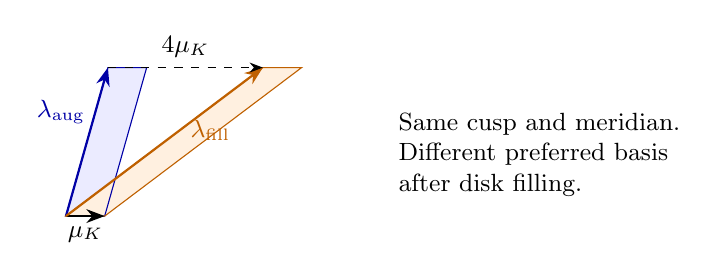
\begin{tikzpicture}[>=Stealth,scale=.82,font=\small]
\coordinate (O) at (0,0);\coordinate (U) at (.6,0);
\coordinate (A) at (.65,2.3);\coordinate (F) at (3.05,2.3);
\fill[blue!8] (O)--(U)--($(U)+(A)$)--(A)--cycle;
\fill[orange!12] (O)--(U)--($(U)+(F)$)--(F)--cycle;
\draw[blue!65!black] (O)--(U)--($(U)+(A)$)--(A)--cycle;
\draw[orange!75!black] (O)--(U)--($(U)+(F)$)--(F)--cycle;
\draw[->,thick] (O)--(U) node[midway,below] {$\mu_K$};
\draw[->,thick,blue!65!black] (O)--(A) node[pos=.7,left] {$\lambda_{\rm aug}$};
\draw[->,thick,orange!75!black] (O)--(F) node[pos=.58,right] {$\lambda_{\rm fill}$};
\draw[->,dashed] (A)--(F) node[midway,above] {$4\mu_K$};
\node[align=left,anchor=west] at (5,.95) {Same cusp and meridian.\\Different preferred basis\\after disk filling.};
\end{tikzpicture}

\caption{The image of the augmented longitude and the preferred filled longitude differ by the integral meridian shear in \eqref{pl:F5}. The example shows $p=1$, $\ell=2$, hence shear four; in general it is $\sum_vp_v\ell_v^2$. Both parallelograms generate the same filled cusp lattice.}
\end{figure}

Write \(o_v=1\) for parallel and \(o_v=-1\) for
opposite strand directions in the fixed physical convention.
Then
\[
 \ell_v^2=2(1+o_v),\qquad
 w_\epsilon=\sum_vo_v\epsilon_v,\qquad
 w(D)=w_\epsilon-2\sum_vo_vp_v.
\]
Consequently

\begin{equation}\label{pl:F6}
\begin{aligned}
 a_{\mathrm{aug}}+\sum_vp_v\ell_v^2
  &=-w_\epsilon-\sum_v\epsilon_v+2\sum_vp_v(1+o_v)\\
  &=-w(D)-\sum_v(\epsilon_v-2p_v)=a(D).
\end{aligned}
\end{equation}

Combining \eqref{pl:T4} with \eqref{pl:F5}--\eqref{pl:F6} proves the squared filled
identity \eqref{pl:T6}, with the original primitive slopes and
preferred longitude.

\section{The determinant-one sign at the complete filled knot}\label{pl:the-determinant-one-sign-at-the-complete-filled-knot}

The squared identity leaves a two-valued ambiguity. Its sign is
fixed at the actual complete filled knot, rather than chosen
to fit the edge product.

The negative trace of a null-homologous peripheral curve is a known
fact; see Menal-Ferrer and Porti,
\cite[Corollary 3.10]{MFP}.
The frame proof below includes the sign and its compatibility with
the lifts used here.

\subsection{A frame calculation on a once-bordered surface}\label{pl:a-frame-calculation-on-a-once-bordered-surface}

Let \(S\) be a compact connected oriented surface of genus \(g\)
with one boundary component. Embed it in an oriented three-manifold
which has a spin structure. Choose a smooth oriented tangent frame
\((e_1,e_2)\) on \(S\), and complete it by the positive unit normal
\(\nu\). Such a tangent frame exists because a surface with
boundary has trivial tangent bundle.

Pulling back the ambient spin double cover along
\((e_1,e_2,\nu)\) gives a double cover of \(S\).
Its monodromy is a homomorphism
\(H_1(S;\mathbb Z/2)\to\mathbb Z/2\).
Since the single oriented boundary is zero in this homology,
the lift of this chosen frame closes after one boundary circuit.

Now replace the first tangent vector on the boundary by its positive
unit tangent \(t\), and the second by the corresponding inward
tangent normal \(n\). Relative to \((e_1,e_2)\), the
frame \((t,n)\) has winding number

\begin{equation}\label{pl:L1}
\chi(S)=1-2g.
\end{equation}

This is the boundary form of the index formula: extend the outward
boundary normal to a tangent vector field with isolated zeros.
The sum of its indices is \(\chi(S)\); measured in the
global tangent frame, it is the degree of its boundary direction.
The boundary tangent differs from that normal by a fixed quarter
turn, which does not change the degree.

A full \(2\pi\) rotation in the tangent plane is the nontrivial
loop of the oriented three-dimensional frame group. It therefore
changes the sign of a spin lift. Formula \eqref{pl:L1} is odd. It follows
that the boundary-adapted frame

\begin{equation}\label{pl:L2}
(t,n,\nu)
\end{equation}

has an antiperiodic lift: after one boundary circuit its lift
returns to the other sheet.

No choice of spin structure changes this conclusion. The only
possible change was the monodromy of the first global frame,
and that monodromy vanishes on the boundary.

\subsection{Application to a complete hyperbolic knot cusp}\label{pl:application-to-a-complete-hyperbolic-knot-cusp}

Let \(Y\) be the oriented complete finite-volume hyperbolic complement
of a knot in \(S^3\). Take a sufficiently far cusp torus \(T\).
Its preferred longitude \(\lambda\) is primitive and bounds
a Seifert surface in the truncated complement.
Arrange the boundary of the surface to be the straight Euclidean
representative of \(\lambda\) on \(T\), and arrange its
collar to meet \(T\) orthogonally. These changes are made
inside the ordinary product collar of the boundary torus.

Along that boundary, \eqref{pl:L2} is a translation-invariant horospherical frame, up to
one constant rotation: \(t\) is the constant longitude
direction, \(n\) is the radial direction, and \(\nu\)
is the constant perpendicular direction in the horosphere.
Thus the preceding surface calculation says that the translation-invariant horospherical frame has
antiperiodic spin holonomy along \(\lambda\).

For precision, identify the oriented frame bundle of hyperbolic
three-space with \(\mathrm{PSL}_2(\mathbb C)\), and its
spin cover with \(\mathrm{SL}_2(\mathbb C)\).
Conjugate the cusp fixed point to infinity. If the longitude
translation is \(z_\lambda\ne0\), the path of translation-invariant
horospherical frames is represented by

\begin{equation}\label{pl:L3}
U(t)=
 \begin{pmatrix}1&t z_\lambda\\0&1\end{pmatrix},
                         \qquad 0\le t\le1.
\end{equation}

This is the lift starting at the identity.
Here translation-invariant refers to the cusp's Euclidean translation
group; no assertion of Levi-Civita parallel transport along a
horocycle in hyperbolic three-space is needed.
For a determinant-one holonomy lift \(\widetilde\rho\),
the endpoint of \eqref{pl:L3} closes in the quotient spin bundle precisely
when
\(\widetilde\rho(\lambda)=U(1)\).
It returns to the opposite sheet precisely when
\(\widetilde\rho(\lambda)=-U(1)\).
The antiperiodicity just proved therefore gives

\begin{equation}\label{pl:L4}
\boxed{\displaystyle
 \widetilde\rho(\lambda)=
       -\begin{pmatrix}1&z_\lambda\\0&1\end{pmatrix},
 \qquad
 \operatorname{tr}\widetilde\rho(\lambda)=-2.}
\end{equation}

Reversing the longitude replaces this matrix by its inverse and
does not change the sign. Any two determinant-one lifts differ
by a character to \(\{\pm1\}\), and the preferred longitude
is zero in the knot complement's first homology, so \eqref{pl:L4} is
independent of that choice as well.

Here spin existence needs no general three-manifold theorem.
Remove a point of the knot from \(S^3\); its complement is
\(\mathbb R^3\), whose standard tangent frame restricts to \(Y\).
Orthonormalizing for the hyperbolic metric gives a spin structure
on its oriented frame bundle and hence a lift of its geometric
holonomy. The sign calculation itself is the explicit surface-frame
argument above.

\subsection{Compatibility with the original augmented representation}\label{pl:compatibility-with-the-original-augmented-representation}

Return to the original all-circle construction. Write
\(\mu_K\) for its main meridian and \(\mu_v\) for its
original auxiliary meridians. The original circles are pairwise
unlinked. If \(\ell_v\) is the linking number of circle
\(v\) with the main knot and \(p_v\) is its integral
filling coefficient, the fixed main-boundary word which becomes
the preferred filled longitude is

\begin{equation}\label{pl:L5}
\lambda_{\mathrm{fill}}
       =\lambda_K\mu_K^{\sum_vp_v\ell_v^2}.
\end{equation}

In the augmented exterior its first homology class is

\begin{equation}\label{pl:L6}
[\lambda_{\mathrm{fill}}]
      =\sum_v\ell_v[\mu_v]
           +\sum_vp_v\ell_v^2[\mu_K].
\end{equation}

The original crossing disk is punctured by exactly two main
strands, so

\begin{equation}\label{pl:L7}
\ell_v\in\{0,2,-2\}.
\end{equation}

Consequently \eqref{pl:L6} vanishes modulo two.

At an actual complete filled knot point, pull back any
determinant-one lift of its complete holonomy to the augmented
group. Locally this lift continues through the augmented geometric
family: lift the finitely many generator matrices holomorphically;
the signs of the finitely many relations are discrete and remain
their identity values at the initial point.
If another local determinant-one lift is used for the face
construction, its ratio with this lift is a
\(\{\pm1\}\)-valued character: both project to the same
projective representation after one fixed conjugation.
By \eqref{pl:L6}--\eqref{pl:L7}, that character is one on
\(\lambda_{\mathrm{fill}}\).
Thus any such local face-map lift has exactly the same longitude
sign as the filled lift in \eqref{pl:L4}. A globally rational
determinant-one lift over the entire source variety is not
assumed or needed.

This step is useful because the original matrices of an auxiliary
filling slope may be \(-I\) rather than \(I\). One need not
assume that the particular auxiliary lifts descend to the filled
group. Their possible discrepancy is a character and cannot
change \eqref{pl:L5}.

\subsection{Fixing a holomorphic squared longitude identity}\label{pl:fixing-a-holomorphic-squared-longitude-identity}

The squared identity proved above, on a connected geometric germ
with the original selected main flag and fixed filling equations, is

\begin{equation}\label{pl:L8}
L_{\mathrm{geom}}^2
     =M^{2a(D)}
          \prod_e\left(\frac{M^2-X_e}{1-M^2X_e}\right)^2.
\end{equation}

The factors are holomorphic units near its complete filled point. Define
the longitude coordinate as the inverse eigenvalue on the source
\(M^{-1}\) meridian line. The ratio of the two sides before
squaring is then a holomorphic function taking values in
\(\{1,-1\}\); it is constant on the connected germ.

At the actual complete filled point, \(M=1\).
Each edge factor in \eqref{pl:L8} is one, since the geometric wire does
not have \(X_e=1\). The inverse selected longitude eigenvalue
is \(-1\) by the preceding complete-cusp and lift comparison. Therefore the constant is negative:

\begin{equation}\label{pl:L9}
\boxed{\displaystyle
 L_{\mathrm{geom}}
       =-M^{a(D)}
          \prod_e\frac{M^2-X_e}{1-M^2X_e}.}
\end{equation}

The conclusion requires the exact squared identity as input.
The complete-value sign fixes only its remaining two-valued
ambiguity; it is not being used to infer the dependence on \(M\)
or on any auxiliary parameter.

\noindent This completes the proof of Theorem~\ref{pl:all-circle}.

\section{The literal insertion}\label{plb:the-literal-insertion}

Use the reduced tree of original product junctions, with consecutive unturned products already grouped. A bare vertex has full valence at least three. Its incident edges are the original quarter-turns; a binary resolution used to describe its positive kernel does not add physical edges.

At a bare vertex insert the literal unturned box \(R^0=I\), at the distinguished position immediately before the original ordered child product. Encircle its two strands by a new crossing circle. Keep every child in its original order. Put

\begin{equation}\label{plb:1}
\epsilon_v=p_v=n_v=0
\end{equation}

at this new circle. Filling its original primitive meridian removes the auxiliary circle and restores the literal identity box. Thus the filled tangle, its endpoints, its framed main strands and its original peripheral curves are unchanged. No new quarter-turn is inserted. Repeating the operation at all bare vertices produces a literal all-circle tree on the same physical edge set.



\begin{figure}[tb]
\centering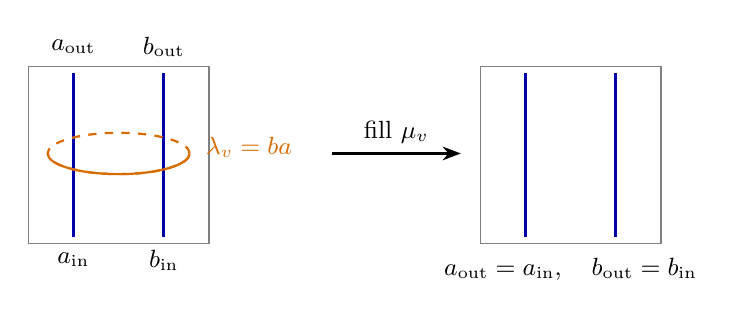
\begin{tikzpicture}[>=Stealth,font=\small,scale=.82]
\begin{scope}
 \draw[gray] (-.7,-.1) rectangle (2.1,2.65);
 \draw[very thick,blue!65!black] (0,0)--(0,2.55) (1.4,0)--(1.4,2.55);
 \draw[orange!85!black,thick,dashed] (.7,1.3) ellipse (1.1 and .32);
 \draw[orange!85!black,thick] (-.4,1.3) arc[start angle=180,end angle=360,x radius=1.1,y radius=.32];
 \node at (0,-.35) {$a_{\rm in}$};\node at (1.4,-.35) {$b_{\rm in}$};
 \node at (0,2.95) {$a_{\rm out}$};\node at (1.4,2.95) {$b_{\rm out}$};
 \node[orange!85!black,anchor=west] at (1.9,1.4) {$\lambda_v=ba$};
\end{scope}
\draw[->,thick] (4,1.3)--(6,1.3) node[midway,above,align=center] {fill $\mu_v$};
\begin{scope}[xshift=7cm]
 \draw[gray] (-.7,-.1) rectangle (2.1,2.65);
 \draw[very thick,blue!65!black] (0,0)--(0,2.55) (1.4,0)--(1.4,2.55);
 \node at (.7,-.5) {$a_{\rm out}=a_{\rm in},\quad b_{\rm out}=b_{\rm in}$};
\end{scope}
\end{tikzpicture}

\caption{A new circle surrounds the two straight strands in the fixed product collar. Its disk longitude retains the ordered word $ba$. Meridian filling deletes the circle and restores the same framed collar, with the same access paths. This is a filling operation, not an isotopy of the unfilled exteriors.}
\end{figure}

The fixed access paths make these ordered equalities precise. They
are constructed in Section~\ref{plb:what-the-edge-equations-see-at-the-complete-bare-representation}; the figure records the collar without
choosing additional paths.

For a holonomy representation, the added meridian must be projectively
identity: its matrix must be a scalar. An eigenvalue ratio of one would
also permit a nontrivial parabolic matrix. Section~\ref{plb:a-unique-regular-zero-power-angular-saddle} excludes this
ambiguity by exhibiting an auxiliary longitude with distinct eigenvalues.

The original crossing powers, writhe and integer

\begin{equation}\label{plb:2}
a(D)=-w(D)-\sum_v n_v.
\end{equation}

are unchanged. The added circles have filling parameter zero, so their preferred-longitude surgery correction \(p_v\ell_v^2\) also vanishes.



After the zero-power circles have been inserted, the
ordered all-circle cut of \cite{Nonparabolic}
joins the edge blocks in the original page order. The labels fix every attachment.
The representation comparison below also permits a flat added
subdivision; it uses the original strict geometry to identify the knot
holonomy.

\section{A unique regular zero-power angular saddle}\label{plb:a-unique-regular-zero-power-angular-saddle}

Let a bare hub have \(m\ge3\) incident covariant labels \(x_1,\ldots,x_m\), with

\begin{equation}\label{plb:3}
0<x_j\le\tfrac12,\qquad
 \#\{j:x_j=\tfrac12\}\le1,\qquad
                         \sum_jx_j>1.
\end{equation}

Here is the complete-state window needed for this assertion; it is a
classical consequence of the stationary profiles, not an analytic source
estimate. Remove the original circle operators at the complete state.
An exposed circle-side profile is $g(a)+c$, where
$g(a)=J(2a)-4J(a)$, by \cite[Proposition 4.2]{Profiles}.
Consider a connected bare component with these profiles at its external
incidences. At any rooted ordinary output $b$ put
\[
 B=\cot\pi b,\quad \kappa=e^{-f'(b)},\quad
 X^2=\frac{1+B^2}{1+\kappa},\quad Y^2=\kappa X^2.
\]
The stationary product and turn formulas of \cite[Lemma 4.1]{Profiles}
are
\[
 B_o=\frac{B_1B_2+X^2-1}{B_1+B_2},\quad
 Y_o=\frac{Y_1Y_2}{B_1+B_2},\quad
 B_1+B_2>0,\qquad (B,X,Y)\longmapsto(-B,Y,X).
\]
Rigid inputs have $(B,B,1)$, and every composite input is proper:
$-Y<B<X$. At the last binary product, strict support gives
$B_o<B_i\le X$. The identity
\[
 Y_o^2=(B_1-B_o)(B_2-B_o)\le(X-B_o)^2
\]
therefore implies
\[
 X\ge X_2(B_o):=\frac{B_o+\sqrt{B_o^2+2}}2,
 \qquad f'(b)\ge 2\log(2X_2(\cot\pi b)^2).
\]
The inequalities are strict if either child is composite. In particular
$f'(b)>0$ for $b<1/2$, and $f'(1/2)\ge0$, with equality only for the
single trivalent hub with two rigid external inputs. The equality
profile $f_2+c$ is symmetric under $b\mapsto1-b$, since
$X_2(B)X_2(-B)=1/2$.

Cut a physical edge between bare hubs. Its full pressure is
$f_A(1-x)+f_B(1-x)$, so it strictly decreases for $x>1/2$.
At $x=1/2$ its derivative is strictly negative unless both sides are
single trivalent hubs with two rigid external inputs. In that exception
it is $2f_2(1-x)+c$ and strict concavity makes its unique maximum
$x=1/2$. Edges incident to a circle have $0<x<1/2$ by the strict leaf
interval after exposing that incidence. Hence only the indicated
internal edge can reach half, and at most one such edge meets a hub.
Finally the exact whole-hub support in \cite[Lemma 2.4]{Profiles} is
$x_i+x_j<1$ and $\sum_jx_j>1$, so it supplies the last condition
of \eqref{plb:3}. Hidden binary-resolution labels are not physical edges.


The angular variable \(\tau\) describes the auxiliary disk longitude
by \(Q=e^{i\tau}\). The
circle-incidence action
is

\begin{equation}\label{plb:4}
b(x,\tau)=\int_0^x
       \log(2\cos(2\pi r)+2\cos\tau)\,dr-2J(x),
 \qquad J'(x)=\log(2\sin\pi x).
\end{equation}

Here \(J(0)=0\); its derivative specifies its continued branch. For \(\tau=-iy\), \(y>0\), every logarithm in the integral is real and finite. Put \(k=\tanh(y/2)\). Direct integration gives

\begin{equation}\label{plb:5}
b_\tau(x,-iy)=\frac{i}{\pi}
             \arctan\bigl(k\tan(\pi x)\bigr),
 \quad 0<x<\tfrac12,
\end{equation}

with value \(i/2\) at \(x=1/2\). Indeed
\[
 \int_0^x\frac{\sinh y}{\cosh y+\cos2\pi r}\,dr
   =\frac1\pi\arctan\bigl(k\tan\pi x\bigr).
\]
The zero-power first-charge equation is therefore

\begin{equation}\label{plb:6}
\sum_jb_\tau(x_j,\tau)-i=0
 \quad\Longleftrightarrow\quad
 \sum_j\arctan(k\tan\pi x_j)=\pi.
\end{equation}

A half label contributes \(\pi/2\). The left side is strictly increasing for \(0<k<1\), starts at zero or \(\pi/2\), and tends to \(\pi\sum_jx_j>\pi\). Thus \eqref{plb:6} has exactly one solution \(0<k<1\). Consequently

\begin{equation}\label{plb:7}
y=2\operatorname{arctanh}k>0,\qquad
 Q=e^{i\tau}=e^y=\frac{1+k}{1-k}>1.
\end{equation}

At least two labels are strictly below half. Differentiating \eqref{plb:6} shows that its derivative is strictly positive, so the angular Hessian is nonzero. The saddle and its selected logarithms extend holomorphically to a complex neighborhood of the fixed label tuple. The half-label case causes no singularity: the integrand of \eqref{plb:4} remains nonzero at \(y>0\), and \eqref{plb:6}'s derivative still has the contributions of the other labels.

In particular the new auxiliary longitude has distinct eigenvalues. If its meridian has similarity one and commutes with that longitude, it is projectively identity. The possible unipotent ambiguity at \(Q^2=1\) is absent.

\section{Exact elimination of the angular action}\label{plb:exact-elimination-of-the-angular-action}

Let \(V_m(\mathbf x)\) be the complete positive action of the whole hub.
It is defined by the ordered product kernel of \cite{Profiles}: resolve the original ordered product by any fixed binary association, sum its cubic gate actions, and optimize the hidden complementary labels. The conditional optimizer is strict and has negative definite Hessian on the strict whole-hub support.

Then on \eqref{plb:3},

\begin{equation}\label{plb:8}
V_m(\mathbf x)=
 \underset{\tau}{\operatorname{stat}}
       \left\{\sum_jb(x_j,\tau)-i\tau\right\},
 \qquad \tau=-iy \text{ from \eqref{plb:6}}.
\end{equation}

The equality includes its constant.

Here is one derivation retaining the exact complete normalization. The Newton factors are the finite polynomial basis used for the
tangle evaluation. For a factor with normalized index \(0<x<1/2\),
the logarithm of its Laurent coefficient at normalized exponent \(r\),
divided by the level, has rate

\begin{equation}\label{plb:9}
B_x(r)=J(2x)-2J(x)-J(x+r)-J(x-r),\qquad |r|\le x.
\end{equation}

To see exactly which finite equality is used, set
$S_r=\prod_{j=1}^r2\sin(\pi j/N)$ and
\[
 e_n(z)=S_n^{-2}\prod_{j=0}^{n-1}
       (2\cos((2j+1)\pi/N)-z),\qquad n<N/2.
\]
The finite sine-binomial identity gives
\[
 e_n(-u-u^{-1})=\sum_{r=-n}^n
 \frac{S_{2n}}{S_n^2S_{n+r}S_{n-r}}u^r.
\]
All coefficients are positive. For a fixed number $m$ of factors,
write their convolution coefficients $a_r$, and put
$d_\ell=a_{\ell N-1}-a_{\ell N+1}$. The exact complete top trace is
\[
 \phi_0\Bigl(\prod_j e_{n_j}\Bigr)
 =N^2\sum_{\ell\ge1}(-1)^{(N-1)(\ell+1)}\ell d_\ell.
\]
This is the finite Fourier formula of \cite[Lemma 6.1]{SourceBounds};
it is the same positive binary-resolution trace obtained from
\cite[Proposition 3.2 and Theorem 3.3]{Newton}.
The primitive internal coefficient lattice makes the latter's logarithmic
rate precisely $V_m$ by finite Laplace summation.

For completeness, no cancellation assertion about a knot invariant is
needed to extract the rate on the other side. Take $n_j/N\to x_j<1/2$
with $\sum x_j>1$. The sine-factorial estimate
of \cite[Lemma 5.2]{Newton} gives the uniform coefficient
rate $B_{x_j}(r)$ in \eqref{plb:9}, with $O(\log N)$ errors, including
the endpoints. Rounding a constrained maximizing tuple while preserving
its total gives
\[
 N^{-1}\log a_{k}\longrightarrow
 \mathcal B(k/N),\qquad
 \mathcal B(s)=\max_{\sum r_j=s}\sum_jB_{x_j}(r_j).
\]
Uniformly on a compact neighborhood of this strict tuple,
$B_x''(r)=-\pi\sin(2\pi x)/[\sin\pi(x+r)\sin\pi(x-r)]$
is bounded above by a negative constant. Thus $\mathcal B$ is even
and strongly concave, and its values at integers $\ell\ge2$ are
strictly below $\mathcal B(1)$.
Each factor's coefficient sequence is symmetric unimodal. Decompose it
into nonnegative multiples of interval indicators. For an interval
convolution of $m$ factors with radii at most $M_N=\lfloor(N-1)/2\rfloor$,
its nonzero count at $k\ge M_N$ strictly drops by step two, and that
integer drop is at least one; the count is at most $(2M_N+1)^m$.
Here is the counting argument. Let $r$ be the largest interval radius
and write its convolution as $C=\mathbf1_{[-r,r]}*H$. Then
$C(k)-C(k+1)=H(k-r)-H(k+r+1)$. If $k\ge r$ and $C(k)>0$,
$k-r$ lies in the interval support of $H$. If $k+r+1$ is outside
that support, the difference is positive. Otherwise $k+r$ lies
in the support and is at least every radius occurring in $H$.
Induction on the number of intervals gives
$H(k+r)>H(k+r+1)$; unimodality gives $H(k-r)\ge H(k+r)$.
The one-interval case is immediate. Thus the step-one decrease,
and hence the step-two decrease, is a positive integer in this range.
Summing the decompositions gives
$a_{N-1}\le N^m d_1$. Thus $d_1>0$ has rate $\mathcal B(1)$,
whereas the finitely many $d_\ell$ with $\ell\ge2$ are exponentially
smaller. The displayed alternating finite trace therefore has rate
\begin{equation}\label{plb:10}
 V_m(\mathbf x)=\max_{\substack{\sum_jr_j=1\\ |r_j|\le x_j}}
                              \sum_jB_{x_j}(r_j).
\end{equation}
This uses only the finite trace and scalar sine products. It is
independent of all quantum asymptotic and filled-volume theorems.

For \(0<x<1/2\),
\[
 B_x'(r)=\log\frac{\sin\pi(x-r)}{\sin\pi(x+r)}.
\]
The unique maximizer of \(B_x(r)+yr\) is

\begin{equation}\label{plb:11}
r=\frac1\pi\arctan\bigl(\tanh(y/2)\tan\pi x\bigr).
\end{equation}

Moreover

\begin{equation}\label{plb:12}
b(x,-iy)=\max_{|r|\le x}\{B_x(r)+yr\}.
\end{equation}

To verify the constant, at \(y=0\) both sides are
\(J(2x)-4J(x)\). Their \(y\)-derivatives are the same \(r\) by \eqref{plb:5} and \eqref{plb:11}. The constrained maximizer \eqref{plb:10} has common multiplier \(y>0\), determined by \(\sum r_j=1\). Equations \eqref{plb:10}--\eqref{plb:12} prove \eqref{plb:8}. A half label follows by continuity. Equivalently \(B_{1/2}(r)=0\), so its tilted maximum is \(y/2\), as also follows directly from \eqref{plb:4}.

For a cubic vertex one can avoid the finite trace altogether. The old action is

\begin{equation}\label{plb:13}
t(x_1,x_2,x_3)=
 \sum_{i<j}J(x_i+x_j)-\sum_iJ(x_i)-J(x_1+x_2+x_3-1).
\end{equation}

Writing \(a_j=\tan\pi x_j\), equation \eqref{plb:6} gives
\(k^2=(a_1+a_2+a_3)/(a_1a_2a_3)\).
The derivative of the right side of \eqref{plb:8} in \(x_j\) is

\begin{equation}\label{plb:14}
\log\frac{\cosh y+\cos2\pi x_j}{2\sin^2\pi x_j}
   =\log\frac{k^2+\cot^2\pi x_j}{1-k^2},
\end{equation}

which is exactly \(\partial_jt\). As \(\sum x_j\downarrow1\), \(y\to\infty\), and both actions tend to \(-2\sum_jJ(x_j)\). This proves the cubic identity with its absolute constant.

Both sides of \eqref{plb:8} are holomorphic near the fixed strict tuple. Their equality on an open real set proves equality of the continued germs. At the possible half label, use their holomorphic continuation from labels below half; both Hessians remain invertible there.

\section{The actual added longitude in the old prism geometry}\label{plb:the-actual-added-longitude-in-the-old-prism-geometry}

The previous section identifies actions. The following matrix calculation identifies the new circle inside the
original marked geometry. A white map is the full Möbius transition
between a white face in one projection copy and its partner in the
other copy. Its translation as well as its fixed points is retained.

At an ordinary output face of the bare product write
\[
 E=e^{2\pi ib},\qquad R=\frac1{1+\kappa},\qquad
 \kappa=e^{-f'(b)}.
\]
The marked construction \cite[Section 7]{StrictGeometry}
gives the universal white maps

\begin{equation}\label{plb:15}
W_1=\begin{pmatrix}1&E-1\\0&E\end{pmatrix},\qquad
 W_3=\begin{pmatrix}R&0\\1-E&ER\end{pmatrix}.
\end{equation}

They are the top and bottom white-face maps at a bare product. Through every original binary product, the full matrix identities give

\begin{equation}\label{plb:16}
W_{F,1}=W_{G,1}=W_{o,1},\qquad
 W_{F,3}=W_{G,3}=W_{o,3}
\end{equation}

in the common coordinate frame. Consequently the same ordered side word is seen at every boundary face of that hub.

Insert the zero-crossing box in the original disk frame. Its primitive disk-longitude path crosses these two white sides, giving \(W_1^{-1}W_3\), up to the inversion required when the circle's orientation is reversed. The determinant-one normalization is

\begin{equation}\label{plb:17}
P=\frac1R W_1^{-1}W_3,\qquad
 \operatorname{tr}P
   =2-\frac{4\sin^2\pi b}{R}.
\end{equation}

This is the same \(W_1^{-1}W_3\) disk word used at the corresponding end of an all-circle edge; it is not a trace chosen to fit \eqref{plb:6}.

The response metric records the ordered quadrilateral shape at a
product boundary. Its coordinate \(X_{\mathrm{met}}\) is distinct
from the exponential wire variable \(X_e=e^{2\pi ix_e}\). It is
\[
 X_{\mathrm{met}}^2=\frac{1+\cot^2\pi b}{1+\kappa}.
\]
Therefore

\begin{equation}\label{plb:18}
\operatorname{tr}P=2-\frac4{X_{\mathrm{met}}^2}.
\end{equation}

At a boundary incidence with covariant label \(x\), the ordinary output is \(b=1-x\), and the conditional action satisfies \(f'(b)=-\partial_xV_m\). Using \eqref{plb:14}, valid at any valence by the envelope identity \eqref{plb:8}, gives

\begin{equation}\label{plb:19}
X_{\mathrm{met}}^2
 =\frac1{\sin^2\pi x\,[1+\exp(\partial_xV_m)]}
 =\operatorname{sech}^2(y/2)=1-k^2.
\end{equation}

Thus

\begin{equation}\label{plb:20}
\operatorname{tr}P=-2\cosh y=-(Q+Q^{-1}).
\end{equation}

This proves that the actual added longitude has the regular eigenvalues required by the angular saddle. The proof retains the old group word, and shows why a bare hub has a common \(Q\) across all its pages.

When an incidence is viewed through its physical turn, the old identity
\(T W_{j+1}(E,R)=W_j(E^{-1},1-R)T\)
takes the \(W_1^{-1}W_3\) word to the appropriate inverse of the \(W_2^{-1}W_0\) word. Its trace is unchanged. The auxiliary flag may be selected on the eigenvalue \(-Q\), \(Q>1\); the main meridian flags are not changed by this auxiliary choice.

\section{What the edge equations see at the complete bare representation}\label{plb:what-the-edge-equations-see-at-the-complete-bare-representation}

Pull the original complete holonomy back along the exact filling quotient obtained in Section~\ref{plb:the-literal-insertion}. This gives a representation of the enlarged augmented link with every newly added meridian equal to identity. It is a representation-theoretic pullback; no assertion that the drilled link carries this metric is needed.

\subsection{The marked zero-crossing collar}\label{plb:the-marked-zero-crossing-collar}

Choose the box in a framed ball \(D^2\times[0,1]\), with its two strands
\(\{p_1,p_2\}\times[0,1]\). Choose a basepoint \(z_*\in\partial D^2\),
an ordered pair of disjoint access paths from it to small circles around
\(p_1,p_2\), and transport that entire system by the product framing.
Orient and name the resulting based puncture loops \(a,b\) so that
the oriented disk-boundary word is \(ba\). The boundary basepath is
\(\{z_*\}\times[0,1]\). Transport across this literal zero-crossing box gives

\begin{equation}\label{plb:22c}
a_{\mathrm{out}}=a_{\mathrm{in}},\qquad
                        b_{\mathrm{out}}=b_{\mathrm{in}}.
\end{equation}

These are equalities in the based fundamental group, before taking any
representation. No permutation of punctures, turn of an access path,
or power of the disk-boundary curve is included.

Place the new auxiliary circle at the disk boundary in the middle
of this collar, with the original disk framing. Its longitude is
the parallel copy of that boundary and retains the based word \(ba\).
The meridian filling deletes the auxiliary circle and returns exactly
the framed collar just described. Its quotient on fundamental groups
fixes \(a,b\), their access paths, and the boundary basepath. Thus it
also fixes the ordered maps by which this collar is joined to all
earlier and later product factors. This remains true when there are
several child factors: transport the same system through them in
their recorded order. It never requires the factors to commute.

For comparison with a pair of projection faces, transport the framed
loops to the face basepoints along the original specified paths.
If the old transport is \(C_0\), \eqref{plb:22c} becomes the simultaneous
conjugacy \(C_0aC_0^{-1}=a'\), \(C_0bC_0^{-1}=b'\).
Reading the other side of a puncture changes the corresponding
native generator to its inverse. Those inversions are recorded
explicitly in \eqref{plb:22b} below; they do not change \eqref{plb:22c} into a braid.
This is the marked van Kampen statement used at every added seam.
Only a retained nonzero half twist changes \eqref{plb:22c}, by the separately
calibrated Hurwitz action.

Each boundary chart here is the ordered quadrilateral supplied by the
original cell construction. It is not assumed to be a new
four-punctured topological boundary. On a physical turn edge use its
original coordinate \((0,\infty,1,R)\) and its phase \(E=e^{2\pi ix}\).
This is the transported physical-edge frame from the last paragraph
of Section~\ref{plb:the-actual-added-longitude-in-the-old-prism-geometry}; its phase is the reciprocal of the ordinary-output
phase \(e^{2\pi ib}\), with the corresponding change \(R\mapsto1-R\).
At \(M=1\) the four native all-circle white matrices of \cite{Nonparabolic} are exactly the universal old \(W_j(E,R)\), projectively. This follows by putting \(m=1\) in the explicit native chart, without specializing the auxiliary eigenvalues to one.

The two disk words have normalized traces \(-\beta,-\gamma\), where

\begin{equation}\label{plb:21}
\beta=\frac{2R-(E+E^{-1})}{1-R},\qquad
 \gamma=\frac{2-(E+E^{-1})-2R}{R}.
\end{equation}

At an inserted hub these are supplied by \eqref{plb:20}; at an original circle they are its original marked longitude trace. Eliminating \(R\) yields

\begin{equation}\label{plb:22}
A=\frac{4-\beta\gamma}{\beta+\gamma+4},
 \qquad A=E+E^{-1},
\end{equation}

which is exactly the all-circle edge equation at \(M=1\). Thus the old phase is one of its two reciprocal roots. The native white maps retain \(E\) itself, not just \(E+E^{-1}\); the existing native/character comparison identifies the all-circle source variable with that \(E\).

All character-chart denominators are units at this point: \(\beta,\gamma\ge2\), \(E\ne1\), and the displayed quadrilateral vertices are distinct. The allowed value \(E=-1\) on the two-hub half edge does not cause a character-matrix singularity. In that case the edge quadratic may ramify over its endpoint parameters; one must use the full stationary branch or another local coordinate, not assert that \(E\) is a simple quadratic root.

Indeed \(E=-1\) gives

\begin{equation}\label{plb:22e}
(\beta-2)(\gamma-2)=16
 \quad\Longleftrightarrow\quad
 X_{\mathrm{met},v}^{\,2}+X_{\mathrm{met},w}^{\,2}=1,
\end{equation}

by \eqref{plb:18}. This is the possible half-edge fold of the old geometry.
The normalized matrices and the two irreducible puncture pairs
below remain regular there.

Here is the boundary-group comparison, including the tuple that has to be retained. First choose the normalized native matrix representatives for the four old projective white maps. In terms of the raw universal representatives used in \eqref{plb:15}, their scalar factors are respectively

\begin{equation}\label{plb:22d}
E^{-1},\quad E^{-1},\quad
                [E(1-R)]^{-1},\quad (ER)^{-1}.
\end{equation}

Each normalized matrix has determinant \(E^{-1}\) at \(M=1\).
The raw universal representatives do not all have that determinant:
in particular the factors involving \(R\) and \(1-R\) cannot be
discarded when taking an SL trace. With \(W_j\) now denoting these
normalized native representatives, put in each original edge frame

\begin{equation}\label{plb:22a}
N_j=W_{j-1}^{-1}W_j,\qquad
 (A,B,C,D)=(N_3,N_0,N_1,N_2)
\end{equation}

with the subsequent determinant-one puncture normalizations from the
all-circle chart. These subsequent powers of \(M\), not the scalar
factors in \eqref{plb:22d}, are one at \(M=1\). Thus every \(N_j\) has determinant
one and trace two. The actual page table is

\begin{equation}\label{plb:22b}
\begin{array}{c|c|c|c}
\text{end}&(a,b)&(a',b')&ba=b'a'\\ \hline
v&(B,A)&(C^{-1},D^{-1})&AB\\
w&(B^{-1},C^{-1})&(A,D)&(BC)^{-1}.
\end{array}
\end{equation}

The entries refer to paths, with the inverse on each puncture determined by its side of the disk. They are exactly the table of the literal all-circle cut, not a new identification of equal traces.

To apply that table to the old holonomy, first insert the zero-crossing box in the actual diagram, before assigning matrices. The main strands and their ordered endpoint paths are unchanged. Add the new circle and perform the literal projection/disk cut. The filling quotient takes every old main meridian and its old basepath to itself and kills the new circle meridian. In particular the four small corner paths reduce to the original consecutive-white words in \eqref{plb:22a}. A white face split by the added cut retains the same transport on both of its pieces: crossing the extra cut and returning differs by the new meridian, whose image is identity. This is also the full-map invariant \eqref{plb:16} through every prism of the original product. Thus the developed four white transitions of the pulled-back representation are exactly the four \(W_j\) already compared above.

The paths across the added disk pages are still the paths of this cut. By van Kampen they intertwine both generators in the appropriate row of \eqref{plb:22b}, with precisely the displayed inversions; the product column is their original primitive disk boundary. The inserted box has no crossing, so no Hurwitz exchange is made at its distinguished seam. The old retained half twists keep their original exchanges.

At \(M=1\), either input pair in \eqref{plb:22b} is irreducible. Both punctures have trace two, and the products in the two rows have traces \(-\beta\) and \(-\gamma\), respectively, with \(\beta,\gamma\ge2\). Their irreducibility obstructions are \((\beta+2)^2\ne0\) and \((\gamma+2)^2\ne0\). Two intertwiners of either full ordered pair differ by its scalar centralizer. Therefore the pulled-back page transport equals the native pure transport in PGL. At an original odd seam the same argument is applied after the already calibrated full Hurwitz action. The corner flags on the main cusp are the old parabolic flags, and the extra auxiliary flags are chosen from \eqref{plb:20}; these choices do not alter a group generator.

All white and shaded generators of the cut now agree, in their original tree frames. This proves equality of the complete representations, not only of the local character triples or the main-cusp translation. It identifies the selected all-circle algebraic point with the pullback of the original bare-tree holonomy. The newly introduced ideal vertices need not form positive tetrahedra in this pulled-back representation. In particular an edge with \(E=-1\) can make that added subdivision flat. No metric on the enlarged unfilled exterior is asserted or required.

\section{Stationary elimination at a nonparabolic main meridian}\label{plb:stationary-elimination-at-a-nonparabolic-main-meridian}

Let \(t\) be the actual main deformation parameter, \(M=e^{\pi it}\).
In the existing strict-tree filtered action it enters only through

\begin{equation}\label{plb:23}
\sum_{e\in\mathcal E_T}
       \{2J(x_e)-J(x_e+t)-J(x_e-t)\}
       +\frac{\pi i a(D)}2t^2.
\end{equation}

It does not enter the old bare tensor action or its hidden resolution wires.

The enlarged all-circle action replaces a bare hub by
\(\sum_jb(x_j,\tau_v)-i\tau_v\), with \(n_v=0\).
Eliminating \(\tau_v\) by \eqref{plb:8} returns exactly the old whole-hub action, including its constant, for complex physical wires in the regular neighborhood. The edge set and \eqref{plb:23} do not change, and neither does \(a(D)\). Hence the two full critical-value germs are equal after stationary elimination.

The stationary equations are the original marked ones. Indeed,
\[
 \begin{aligned}
 &\exp\!\left(\partial_x\{b(x,\tau_v)+b(x,\tau_w)
             +2J(x)-J(x+t)-J(x-t)\}\right)\\
 &\qquad=\frac{(X+Q_v)(X+Q_v^{-1})(X+Q_w)(X+Q_w^{-1})}
 {(X-1)^2(1-XM^2)(1-X/M^2)}.
 \end{aligned}
\]
Thus the wire equation is \eqref{pl:T1}. The continued logarithms obey
$\log\rho_{v,e}=-2\pi b_\tau(x_e,\tau_v)$: differentiate in $x_e$
and fix the integration constant at $x_e=0$, where both sides vanish.
The circle equation
$\sum_{e\ni v}b_\tau+\ii n_v\tau_v/(2\pi)-\ii=0$
is consequently exactly $U_v+p_vV_v=-2\pi\ii$, including the original
logarithmic constant. At an added circle it has $p_v=n_v=\epsilon_v=0$.

Here the required nondegeneracy can be checked entirely classically.
Eliminate each added zero-power angle by \eqref{plb:8}. At the original
augmented point all original circle angles are zero and the remaining
wire action is the strict complete action. Its wire Hessian is negative
definite by \cite[Theorem 3.3]{Profiles}. Direct differentiation gives
\[
 b_\tau(x,0)=0,\qquad b_{x\tau}(x,0)=0,\qquad
 b_{\tau\tau}(x,0)=-\frac{\tan\pi x}{2\pi}.
\]
For each original circle put $\eta_v=1/n_v$ and multiply its first-charge
equation by $\eta_v$. At $\boldsymbol\eta=0$ the system is the strict
wire equations together with $\tau_v=0$; its Jacobian is block diagonal,
with the strict wire Hessian and $(\ii/2\pi)I$. The holomorphic
implicit-function theorem gives its unique solution for all sufficiently
small independently signed real $\eta_v$. The unscaled Hessian is
invertible whenever these $\eta_v$ are nonzero, since scaling its circle
rows gives the just-described invertible Jacobian. The equation for
circle $v$ has $\sum b_\tau(x_e,\tau_v)=\tau_v h_v$, with $h_v$
holomorphic, and hence
$\tau_v=2\pi\eta_v/(1-2\pi\ii\eta_v h_v)\ne0$.
These small angles give $Q_v^2\ne1$. Introducing the main parameter
$t$ in \eqref{pl:deformed-action} is a further holomorphic perturbation
of this nonsingular system. All neighborhoods concern a fixed diagram;
no relation between the sizes or signs of its different twists is used.

The new angular Hessian at each bare hub is nonzero. To state the
comparison precisely, first eliminate the old hidden binary-resolution
variables. Their conditional Hessian is invertible by strictness.
Let \(z\) collect the remaining original variables and let
\(\tau_{\mathrm{new}}\) collect only the added angular variables.
The enlarged Hessian has blocks

\begin{equation}\label{plb:23a}
H_{\mathrm{new}}=
 \begin{pmatrix}
 H_{zz}&H_{z\tau}\\ H_{\tau z}&H_{\tau\tau}
 \end{pmatrix},\qquad
 H_{\mathrm{old,red}}
   =H_{zz}-H_{z\tau}H_{\tau\tau}^{-1}H_{\tau z}.
\end{equation}

The block \(H_{\tau\tau}\) is diagonal over the added hubs, with
nonzero entries from \eqref{plb:6}. Equality \eqref{plb:8} identifies its Schur
complement with the old reduced Hessian. The original full Hessian
and its eliminated hidden block are invertible, so
\(\det H_{\mathrm{new}}
 =\det H_{\tau\tau}\det H_{\mathrm{old,red}}\ne0\).
No individual edge Hessian is inverted, including at \eqref{plb:22e}.

The enlarged analytic branch therefore exists with all the original
logarithms retained. Original sufficiently long fillings keep their
auxiliary \(Q_v^2\ne1\); every added zero-power circle has
\(Q_v^2\ne1\) by \eqref{plb:7}, and this persists near the complete branch.

By Section~\ref{plb:what-the-edge-equations-see-at-the-complete-bare-representation} this branch reconstructs the original filled knot representation, rather than only an algebraic solution of the slope eigenvalue equations. Near the old augmented complete point, use the mixed coordinate tuple
consisting of the main meridian logarithm and the original auxiliary
longitude logarithms $V_v=2\log Q_v$. The reconstructed and original
positive families have the same values of this tuple and the same
selected flags. The positive marked gluing theorem therefore identifies
them as nearby representations; equality at the complete point alone
would not suffice. The added zero-circle meridians have already been
killed, so this uniqueness statement is applied on the original augmented
manifold and its positive triangulation. The original sufficiently long filling point lies on that same small branch. There every original filled circle, as well as every added zero circle, has \(Q_v^2\ne1\); the filling words are projectively identity by Section~\ref{plb:a-unique-regular-zero-power-angular-saddle}. The nondegenerate main-meridian branch is then the geometric germ of the original filled knot.

The all-circle squared longitude identity is a rational identity on its integral source variety. It extends to this regular representation, including the half-edge fold, without solving for an individual edge root. The added zero fillings contribute no surgery exponent, the Seifert sign is that of the same original complete knot, and stationary elimination leaves the effective longitude unchanged. Consequently

\begin{equation}\label{plb:24}
L_{\mathrm{geom}}(M)
   =-M^{a(D)}
      \prod_{e\in\mathcal E_T}
                \frac{M^2-X_e(M)}{1-M^2X_e(M)}
\end{equation}

on the original strict-tree filled branch, with \(X_e=e^{2\pi ix_e}\).

This proves Theorem~\ref{pl:strict-longitude} on the geometric germ of the original
filled knot. The same physical edges occur before and after the
zero-circle elimination, and the added circles contribute neither
a crossing power nor a preferred-longitude shear.

The geometric identification uses the full ordered boundary-group
comparison in Section~\ref{plb:what-the-edge-equations-see-at-the-complete-bare-representation}. The equality of actions in Section~\ref{plb:exact-elimination-of-the-angular-action} supplies
the stationary branch, while the marked face maps identify its
representation. These are distinct parts of the proof. This argument supplies no estimate for a quantum invariant or for short fillings.


\section{Reproduction and boundaries of the result}\label{pl:checks}
The accompanying \texttt{check.py} verifies the finite rational identities used in the proof: the edge discriminant and evaluations, character determinants and transports, differential identities, cusp rebasing and sign-sensitive translations, the bare-hub white word, and the integer framing shear. It reduces polynomial identities modulo the actual edge quadratic. It does not establish geometric integrality, the existence of a nonempty algebraic open set, the topological cusp paths, or the analytic implicit-function statements by finite examples; those are the written arguments above. Run the script in a Python environment containing SymPy, with \texttt{--output} followed by a fresh JSON path.

The geometric completion and marked local representation theorem remain the explicit inputs in Proposition~\ref{pl:imports}. Our use of them is independent of quantum asymptotics. All matrices use the same original group and ordered paths. The sign is fixed on an anchored connected germ; the global source identity is squared and makes no choice of a rational determinant-one lift. Short fillings, changing combinatorics and multiple main-component surgery matrices are outside the stated theorem.

\begin{thebibliography}{9}
\bibitem{Nonparabolic} \emph{Nonparabolic holonomy of trees of crossing circles}, companion paper, \href{https://sashakolpakov.github.io/murakamis_dream/papers/nonparabolic-tree-geometry.pdf}{source and proof}.
\bibitem{StrictGeometry} \emph{Marked geometry of strict Conway compositions}, companion paper, \href{https://sashakolpakov.github.io/murakamis_dream/papers/strict-conway-geometry.pdf}{source and proof}.
\bibitem{Profiles} \emph{Stationary profiles of strict Newton trees}, companion paper, \href{https://sashakolpakov.github.io/murakamis_dream/papers/strict-newton-profiles.pdf}{source and proof}.
\bibitem{Newton} \emph{Newton coefficients and positive sources for Conway tangles}, companion paper, \href{https://sashakolpakov.github.io/murakamis_dream/papers/newton-tangles.pdf}{source and proof}.
\bibitem{SourceBounds} \emph{Spectral estimates for Conway tangle sources}, companion paper, \href{https://sashakolpakov.github.io/murakamis_dream/papers/conway-source-bounds.pdf}{source and proof}.
\bibitem{MFP} P. Menal-Ferrer and J. Porti, \emph{Twisted cohomology for hyperbolic three manifolds}, Osaka J. Math. \textbf{49} (2012), 741--769, especially Corollary 3.10. \href{https://doi.org/10.18910/23151}{doi:10.18910/23151}.
\end{thebibliography}
\end{document}
